\documentclass[a4paper,11pt]{article}

% ════════════════════ Kodowanie i język ════════════════════
\usepackage[T1]{fontenc}
\usepackage[utf8]{inputenc}
\usepackage{lmodern}
\usepackage[polish]{babel}

% ════════════════════ Marginesy ════════════════════
\usepackage[margin=2.5cm]{geometry}

% ════════════════════ Matematyka ════════════════════
\usepackage{amsmath}
\usepackage{amssymb}
\usepackage{siunitx}
\sisetup{
	output-decimal-marker = {,},
	per-mode = symbol,
	range-phrase = { -- },
}

% ════════════════════ Grafika i tabele ════════════════════
\usepackage{graphicx}
\usepackage{float}
\usepackage{booktabs}
\usepackage{array}
\usepackage{tabularx}
\usepackage{multirow}
\usepackage{caption}
\usepackage{subcaption}

% ════════════════════ Kolory i linki ════════════════════
\usepackage[dvipsnames]{xcolor}
\usepackage{hyperref}
\hypersetup{
	colorlinks=true,
	linkcolor=NavyBlue,
	citecolor=NavyBlue,
	urlcolor=RoyalBlue,
}

% ════════════════════ Listingi kodu ════════════════════
\usepackage{listings}
\lstset{
	language=C,
	basicstyle=\ttfamily\footnotesize,
	keywordstyle=\color{NavyBlue}\bfseries,
	commentstyle=\color{Gray}\itshape,
	stringstyle=\color{OliveGreen},
	numbers=left,
	numberstyle=\tiny\color{Gray},
	frame=single,
	breaklines=true,
	captionpos=b,
	tabsize=4,
	showstringspaces=false,
}

% ════════════════════ Flowcharty / diagramy ════════════════════
\usepackage{tikz}
\usetikzlibrary{shapes.geometric, arrows.meta, positioning, calc, patterns, decorations.markings}

% ════════════════════ Nagłówek / stopka ════════════════════
\usepackage{fancyhdr}
\pagestyle{fancy}
\fancyhf{}
\fancyhead[L]{\small Bezkontaktowy miernik odległości — Pulse-Phase Ranging}
\fancyhead[R]{\small Wygraj Indeks WETI 2026}
\fancyfoot[C]{\thepage}
\renewcommand{\headrulewidth}{0.4pt}

% ════════════════════ Odstępy ════════════════════
\usepackage{setspace}
\onehalfspacing
\usepackage{parskip}

% ════════════════════ Enumerate customization ════════════════════
\usepackage{enumitem}

% ══════════════════════════════════════════════════════════════
\begin{document}
	
	% ════════════════════ STRONA TYTUŁOWA ════════════════════════════════════════════════════════════════════════════════════════════════════════════════════════════════════════════════════════════════════════════════════════════════════════════════════════════════════════════════════════════════════════════════════════════════════════════════════════════════════════════════════════════════════════════════════════════════════════════════════════════════════
	\begin{titlepage}
		\centering
		\vspace*{1.5cm}
		
		{\Large Ogólnopolski Konkurs Projektowy}\\[0.3cm]
		{\Large\textbf{,,Wygraj Indeks WETI'' --- edycja 2026}}\\[0.2cm]
		{\large Wydział Elektroniki, Telekomunikacji i~Informatyki\\
			Politechnika Gdańska}
		
		\vspace{1.5cm}
		
		{\Huge\bfseries Bezkontaktowy miernik odległości}\\[0.5cm]
		{\Large Metoda hybrydowa Pulse-Phase Ranging\\z~kompensacją temperatury}
		
		\vspace{1.5cm}
		
		% ════════════════════ Schemat blokowy na stronie tytułowej ════════════════════
		\begin{tikzpicture}[
			block/.style={rectangle, draw, fill=NavyBlue!10, minimum width=2.2cm, minimum height=1cm, align=center, font=\small},
			arr/.style={->, >=Stealth, thick},
			scale=0.9, transform shape
			]
			\node[block] (psu) {Zasilanie\\5V$\to$3{,}3V};
			\node[block, right=1.5cm of psu] (tx) {Nadajnik\\TX 40\,kHz\\{\scriptsize (BC817)}};
			\node[block, right=1.5cm of tx] (rx) {Odbiornik\\RX + MCP6002};
			\node[block, right=1.5cm of rx] (mcu) {ATtiny1616\\MCU + AC0};
			\node[block, below=1.0cm of tx] (temp) {Termistor\\NTC};
			
			% Zasilanie -> Nadajnik
			\draw[arr] (psu) -- (tx);
			% Zasilanie -> MCU (górą)
			\draw[arr] (psu.north) -- ++(0,0.5) -| (mcu.north);
			% MCU -> TX burst (górą, niebieski)
			\draw[arr, NavyBlue] (mcu.north east) ++(0,0.2) -- ++(0,0.8) -| node[above, pos=0.25, font=\scriptsize] {Burst 40\,kHz} (tx.north);
			% MCU -> RX sterowanie (PWM)
			\draw[arr] (mcu.west) -- node[below, font=\scriptsize] {PWM} (rx.east);
			% RX -> MCU echo (dołem, czerwony)
			\draw[arr, red] (rx.south east) -- ++(0,-0.5) -| node[below, pos=0.3, font=\scriptsize, text=red] {Echo (ADC)} (mcu.south);
			% Termistor -> MCU
			\draw[arr, gray] (temp.east) -| (mcu.south west);
			\node[gray, font=\scriptsize] at ($(temp.east)+(1.5,-0.3)$) {NTC (ADC)};
			% Fala US
			\draw[arr, blue, thick, loosely dashed]
			(tx.south west) -- ++(0,-0.5) node[below, font=\scriptsize] {Fala US};
		\end{tikzpicture}
		
		\vfill
		
		{\large
			\begin{tabular}{rl}
				\textbf{Autor:}  & Kacper Popko \\
				\textbf{Opiekun:}  & Mateusz Karanowski \\
				\textbf{Szkoła:}  & II Liceum Ogólnokształcące im.\ ks.\ Anny z~Sapiehów \\
				& Jabłonowskiej w~Białymstoku \\
				\textbf{E-mail:}  & kacper@kajpa.pl \\
				\textbf{Data:}    & Marzec 2026 \\
			\end{tabular}
		}
		
		\vspace{1cm}
	\end{titlepage}
	
	% ════════════════════ SPIS TREŚCI ════════════════════════════════════════════════════════════════════════════════════════════════════════════════════════════════════════════════════════════════════════════════════════════════════════════════════════════════════════════════════════════════════════════════════════════════════════════════════════════════════════════════════════════════════════════════════════════════════════════════════════════════════════════════════════
	\tableofcontents
	\listoffigures
	\listoftables
	\newpage
	
	% ══════════════════════════════════════════════════════════════
	% SEKCJA 1: WSTĘP
	% ══════════════════════════════════════════════════════════════
	\section{Wstęp}
	\label{sec:wstep}
	
	Celem projektu jest opracowanie bezkontaktowego miernika odległości spełniającego
	wymagania konkursu ,,Wygraj Indeks WETI 2026''. Urządzenie umożliwia pomiar
	odległości w~zakresie \SIrange{10}{50}{\centi\metre} od obiektu (arkusz kartonu
	$20 \times 20$~\si{\centi\metre}) przy zasilaniu napięciem \SI{5}{\volt}.
	
	Jako metodę pomiarową wybrano \textbf{hybrydową technikę Pulse-Phase Ranging},
	łączącą pomiar czasu przelotu impulsu ultradźwiękowego (ToF) z~pomiarem
	przesunięcia fazowego sygnału echa. Podejście to pozwala uzyskać rozdzielczość
	rzędu \SI{0,1}{\milli\metre} przy jednoczesnym zachowaniu jednoznaczności pomiaru
	w~całym wymaganym zakresie --- łączy zalety obu metod, eliminując ich indywidualne
	ograniczenia.
	
	Projekt kładzie szczególny nacisk na trzy aspekty optymalizacyjne wynikające
	z~kryteriów oceny konkursowej: minimalizację błędu średniokwadratowego (RMSE)
	poprzez zaawansowany algorytm pomiaru fazowego, redukcję poboru mocy dzięki
	agresywnej polityce uśpienia mikrokontrolera oraz minimalizację kosztu
	komponentów przy zachowaniu wysokiej jakości toru pomiarowego.
	
	\subsection{Wymagania konkursowe}
	
	\begin{table}[H]
		\centering
		\caption{Podsumowanie wymagań konkursowych i~kryteriów oceny}
		\label{tab:wymagania}
		\begin{tabular}{lll}
			\toprule
			\textbf{Parametr}       & \textbf{Wartość / Wzór} & \textbf{Max pkt} \\
			\midrule
			Napięcie zasilania      & \SI{5}{\volt}  & --- \\
			Zakres pomiaru          & \SI{10}{\centi\metre} -- \SI{50}{\centi\metre} & --- \\
			Wykrywany obiekt        & Karton $20 \times 20$~\si{\centi\metre} & --- \\
			Błąd RMSE               & Im mniejszy, tym lepiej & 100 \\
			Pobór mocy              & $100 / P_{[\si{\milli\watt}]}$ & 50 \\
			Koszt elementów         & $50 \cdot 50 / C_{[\text{PLN}]}$ & 50 \\
			Jakość projektu         & Uznaniowo (komisja) & 100 \\
			\midrule
			\textbf{Łącznie}        & & \textbf{300} \\
			\bottomrule
		\end{tabular}
	\end{table}
	
	\subsection{Uzasadnienie wyboru metody pomiarowej}
	
	Przed przystąpieniem do projektowania przeanalizowano cztery główne metody
	bezkontaktowego pomiaru odległości pod kątem ich realizowalności na platformie
	ATtiny1616 oraz potencjału punktacyjnego w~konkursie.
	
	\begin{table}[H]
		\centering
		\caption{Analiza porównawcza rozważanych metod pomiaru}
		\label{tab:porownanie_metod}
		\begin{tabularx}{\textwidth}{lcccX}
			\toprule
			\textbf{Metoda} & \textbf{RMSE} & \textbf{Koszt} & \textbf{Złożoność} & \textbf{Uwagi} \\
			\midrule
			Prosty ToF (US)
			& ${\sim}\SI{3}{\milli\metre}$
			& Niski
			& Niska
			& Rozdzielczość ograniczona przez czas narastania obwiedni przetwornika rezonansowego; brak możliwości sub-milimetrowej dokładności \\[6pt]
			\textbf{Pulse-Phase (US)}
			& ${\sim}\SI{0,5}{\milli\metre}$
			& \textbf{Niski}
			& Średnia
			& \textbf{Wybrany kompromis} --- gruby pomiar ToF eliminuje niejednoznaczność fazową, dokładny pomiar fazy daje sub-mm rozdzielczość \\[6pt]
			FMCW chirp (US)
			& ${<}\SI{0,5}{\milli\metre}$
			& Średni
			& Wysoka
			& Wymaga szerokopasmowych przetworników US (${\sim}\SI{30}{PLN}$/para) oraz FFT --- ATtiny1616 z~16\,KB Flash i~2\,KB RAM nie ma wystarczających zasobów \\[6pt]
			Triangulacja optyczna
			& ${\sim}\SI{1}{\milli\metre}$
			& Średni
			& Średnia
			& Wymaga precyzyjnej mechaniki mocowania LED/fotodiody; wrażliwość na oświetlenie otoczenia; trudna powtarzalność prototypu \\
			\bottomrule
		\end{tabularx}
	\end{table}
	
	Metoda Pulse-Phase Ranging została wybrana jako oferująca najlepszy stosunek
	osiągalnej dokładności do złożoności implementacji. Kluczowe argumenty:
	
	\begin{enumerate}[nosep]
		\item Wykorzystuje tanie przetworniki rezonansowe \SI{40}{\kilo\hertz} (koszt pary: ${\sim}\SI{6}{PLN}$).
		\item Algorytm Goertzela do wyznaczania fazy wymaga jedynie ${\sim}\SI{200}{\byte}$ RAM.
		\item Kompensacja temperatury termistorem NTC eliminuje dominujące źródło błędu systematycznego.
		\item Tryb uśpienia ATtiny1616 (Standby z~RTC, $I_{DD} \approx \SI{0,7}{\micro\ampere}$) pozwala osiągnąć średni pobór mocy poniżej \SI{2}{\milli\watt}.
	\end{enumerate}
	
	
	% ══════════════════════════════════════════════════════════════
	% SEKCJA 2: ZASADA DZIAŁANIA
	% ══════════════════════════════════════════════════════════════
	\section{Zasada działania metody Pulse-Phase Ranging}
	\label{sec:zasada}
	
	\subsection{Przegląd metody}
	
	Metoda Pulse-Phase Ranging łączy dwa pomiary wykonywane w~jednym cyklu
	pomiarowym: gruby pomiar czasu przelotu (ToF) oraz dokładny pomiar przesunięcia
	fazowego echa. Takie podejście rozwiązuje fundamentalny problem pomiaru fazowego
	--- niejednoznaczność co $\lambda/2$ --- przy jednoczesnym zachowaniu sub-milimetrowej
	rozdzielczości.
	
	Cykl pomiarowy składa się z~następujących etapów:
	\begin{enumerate}[nosep]
		\item Odczyt temperatury z~termistora NTC (korekcja $v(T)$).
		\item Generacja burstu TX: $N = 8$ cykli sygnału \SI{40}{\kilo\hertz}.
		\item Detekcja początku echa --- pomiar gruby $t_{ToF}$ (timer TCB0).
		\item Próbkowanie sygnału echa w~oknie pomiarowym (ADC0, ${\sim}4$ cykle po ustabilizowaniu się obwiedni).
		\item Obliczenie fazy algorytmem Goertzela --- pomiar dokładny $\varphi$.
		\item Fuzja obu pomiarów i~filtracja wyniku.
		\item Transmisja wyniku przez USART.
		\item Przejście w~tryb Standby (z~RTC wakeup) do następnego cyklu.
	\end{enumerate}
	
	\subsection{Faza 1 --- Pomiar gruby (Time-of-Flight)}
	\label{sec:tof}
	
	Mikrokontroler generuje burst $N = 8$ cykli sygnału prostokątnego o~częstotliwości
	$f_0 = \SI{40}{\kilo\hertz}$ za pomocą timera TCA0 w~trybie Split Mode PWM. Sygnał
	steruje tranzystorem BC817-40, który pobudza nadajnik ultradźwiękowy.
	
	Czas przelotu impulsu do obiektu i~z~powrotem:
	\begin{equation}
		t_{ToF} = \frac{2D}{v(T)}
		\label{eq:tof}
	\end{equation}
	
	gdzie $D$ to odległość od obiektu, a~$v(T)$ to prędkość dźwięku zależna
	od temperatury powietrza. Ściśle: $v(T) = 331{,}3\sqrt{1 + T/273{,}15}$,
	jednak w~zakresie temperatur pokojowych (\SIrange{15}{30}{\celsius})
	aproksymacja liniowa wprowadza błąd poniżej \SI{0,05}{\metre\per\second}
	($< \SI{0,01}{\milli\metre}$ wpływu na pomiar), dlatego stosujemy
	uproszczoną zależność:
	\begin{equation}
		v(T) \approx 331{,}3 + 0{,}606 \cdot T \quad [\si{\metre\per\second}]
		\label{eq:predkosc_dzwieku}
	\end{equation}
	
	Dla zakresu pomiarowego \SIrange{10}{50}{\centi\metre} przy $T = \SI{20}{\celsius}$
	($v \approx \SI{343,5}{\metre\per\second}$):
	\begin{equation}
		t_{ToF,min} = \frac{2 \cdot 0{,}10}{343{,}5} \approx \SI{0,58}{\milli\second}, \qquad
		t_{ToF,max} = \frac{2 \cdot 0{,}50}{343{,}5} \approx \SI{2,91}{\milli\second}
		\label{eq:tof_zakres}
	\end{equation}
	
	Timer TCB0 taktowany zegarem \SI{10}{\mega\hertz} (patrz sekcja~\ref{sec:mcu})
	daje rozdzielczość czasową \SI{100}{\nano\second}, co odpowiada rozdzielczości odległości:
	\begin{equation}
		\Delta D_{tick} = \frac{v(T)}{2 \cdot f_{clk}} = \frac{343{,}5}{2 \cdot 10 \times 10^6} \approx \SI{17,2}{\micro\metre} \text{ / takt}
		\label{eq:rozdzielczosc_tick}
	\end{equation}
	
	Jednak realna rozdzielczość pomiaru grubego jest ograniczona przez czas narastania
	obwiedni sygnału echa. Przetworniki rezonansowe \SI{40}{\kilo\hertz} mają
	dobroć $Q \approx 15$, co oznacza czas narastania obwiedni:
	\begin{equation}
		\tau_{rise} \approx \frac{Q}{\pi f_0} = \frac{15}{\pi \cdot 40000} \approx \SI{0,12}{\milli\second}
		\label{eq:tau_rise}
	\end{equation}
	
	Niepewność momentu detekcji progu obwiedni przekłada się na praktyczną
	rozdzielczość pomiaru grubego rzędu \SIrange{1}{3}{\milli\metre}. To wystarczy
	do jednoznacznego wyznaczenia liczby $n$ półfal w~równaniu (\ref{eq:wynik}),
	ponieważ $\lambda/2 \approx \SI{4,3}{\milli\metre}$.
	
	\subsection{Faza 2 --- Pomiar dokładny (Phase Measurement)}
	\label{sec:phase}
	
	Po detekcji echa mikrokontroler otwiera okno pomiarowe i~próbkuje sygnał
	echo za pomocą ADC0. Z~zebranych próbek obliczane jest przesunięcie fazowe
	$\varphi$ między sygnałem nadawanym (referencyjnym) a~sygnałem echa.
	
	Odległość wynikająca z~pomiaru fazowego:
	\begin{equation}
		D_{fine} = \frac{\varphi}{2\pi} \cdot \frac{\lambda}{2}
		\label{eq:phase}
	\end{equation}
	
	gdzie $\lambda = v(T) / f_0$ to długość fali ultradźwiękowej. Przy
	$T = \SI{20}{\celsius}$:
	\begin{equation}
		\lambda = \frac{343{,}5}{40000} \approx \SI{8,59}{\milli\metre}, \qquad
		\frac{\lambda}{2} \approx \SI{4,29}{\milli\metre}
		\label{eq:lambda}
	\end{equation}
	
	Pomiar fazowy daje niejednoznaczność co $\lambda/2 \approx \SI{4,3}{\milli\metre}$,
	którą rozwiązuje pomiar gruby ToF (sekcja \ref{sec:tof}).
	
	Wynikowa odległość po fuzji obu pomiarów:
	\begin{equation}
		\boxed{D = n \cdot \frac{\lambda}{2} + D_{fine}}
		\label{eq:wynik}
	\end{equation}
	
	gdzie $n = \left\lfloor D_{ToF} / (\lambda/2) + 0{,}5 \right\rfloor$ to liczba
	całkowitych półfal wyznaczona z~pomiaru grubego.
	
	\subsubsection{Weryfikacja spójności wyznaczania \texorpdfstring{$n$}{n} (consistency check)}
	\label{sec:consistency_check}
	
	Wyznaczenie prawidłowej wartości $n$ jest krytyczne dla poprawności fuzji
	pomiarów --- błąd o~$\pm 1$ skutkuje skokiem wyniku o~$\lambda/2 \approx
	\SI{4,3}{\milli\metre}$. Problem pojawia się, gdy reszta $r = D_{ToF}
	\bmod (\lambda/2)$ wpada w~strefę niejednoznaczności blisko granicy
	zaokrąglenia, tj.\ $r \approx 0$ lub $r \approx \lambda/4$.
	
	W~projekcie zastosowano mechanizm weryfikacji: po wyznaczeniu $n$ obliczana
	jest reszta:
	\begin{equation}
		r = D_{ToF} - n \cdot \frac{\lambda}{2}
		\label{eq:consistency_r}
	\end{equation}
	
	Jeśli $|r|$ wpada w~strefę niejednoznaczności ($|r| < \SI{1,5}{\milli\metre}$
	od granicy $\lambda/4 \approx \SI{2,15}{\milli\metre}$, tj.\
	$|r - \lambda/4| < \SI{1,5}{\milli\metre}$), pomiar jest oznaczany jako
	niepewny i~odrzucany. Mikrokontroler powtarza pomiar jednostkowy do 3~razy,
	zanim zgłosi błąd. W~praktyce prawdopodobieństwo trafienia w~strefę
	niejednoznaczności wynosi $2 \cdot 1{,}5 / 4{,}3 \approx \SI{70}{\percent}$
	dla \textit{pojedynczego} pomiaru ToF o~niepewności $\sigma_{ToF} \approx
	\SI{2}{\milli\metre}$, jednak filtr medianowy z~oknem $M = 7$
	(sekcja~\ref{sec:filtr}) skutecznie eliminuje sporadyczne błędy skokowe ---
	nawet jeśli 1--2 z~7 pomiarów jednostkowych mają błędne $n$, mediana
	zwraca wartość poprawną. Połączenie consistency check z~filtrem medianowym
	zapewnia odporność na błędy wyznaczania $n$ bez istotnego wydłużenia
	czasu cyklu pomiarowego.
	
	\subsubsection{Rozdzielczość pomiaru fazowego}
	
	Rozdzielczość pomiaru fazy zależy od rozdzielczości ADC i~stosunku sygnału
	do szumu (SNR). Przy 10-bitowym ADC i~$K$ próbkach na cykl:
	\begin{equation}
		\Delta\varphi_{min} \approx \frac{2\pi}{2^{10} \cdot \sqrt{K/2}} = \frac{2\pi}{1024 \cdot \sqrt{K/2}}
		\label{eq:phase_res}
	\end{equation}
	
	Dla $K = 4$ próbek na cykl ($f_s = 4 \cdot f_0 = \SI{160}{\kilo\hertz}$):
	\begin{equation}
		\Delta\varphi_{min} \approx \frac{2\pi}{1024 \cdot \sqrt{2}} \approx \SI{4,34}{\milli\radian}
	\end{equation}
	
	\textbf{Uwaga dotycząca częstotliwości próbkowania ADC:}
	Datasheet ATtiny1616 określa maksymalną częstotliwość zegara ADC na
	$f_{CLK\_ADC} = \SI{1,5}{\mega\hertz}$ dla pełnej rozdzielczości 10-bitowej.
	Jedna konwersja zajmuje 13 cykli $CLK_{ADC}$, co daje maksymalną częstotliwość
	próbkowania $R_s = 1500000/13 \approx \SI{115}{ksps}$. Wymagana częstotliwość
	$f_s = \SI{160}{\kilo\hertz}$ ($K = 4$ próbki/cykl) wymaga
	$f_{CLK\_ADC} = 160000 \cdot 13 = \SI{2,08}{\mega\hertz}$,
	co przekracza limit dla 10-bit.
	
	Rozwiązanie przyjęte w~projekcie: przy zegarze systemowym $f_{CLK} = \SI{10}{\mega\hertz}$
	(patrz sekcja~\ref{sec:mcu}) i~prescalerze ADC DIV8, częstotliwość zegara ADC wynosi
	$f_{CLK\_ADC} = \SI{10}{\mega\hertz}/8 = \SI{1,25}{\mega\hertz}$ ---
	\textbf{w~pełni w~specyfikacji} dla 10-bitowej rozdzielczości
	(DS, Tab.~36-26: max \SI{1,5}{\mega\hertz}).
	Rejestr ADC0.CALIB zachowuje wartość domyślną DUTYCYC = 1 (25\% duty cycle),
	co jest poprawne dla $f_{CLK\_ADC} \leq \SI{1,5}{\mega\hertz}$
	(DS, sekcja~30.5.17) --- \textbf{eliminuje to konieczność workaround z~DUTYCYC = 0}.
	Maksymalna częstotliwość próbkowania: $R_s = 1250000/13 \approx \SI{96}{ksps}$.
	
	Ponieważ $f_s = \SI{160}{\kilo\hertz}$ przekracza ten limit, przyjęto wariant
	$K = 3$ próbki na cykl z~$f_{CLK\_ADC} = \SI{1,25}{\mega\hertz}$:
	$f_s = 1250000/13 \approx \SI{96}{\kilo\hertz}$, co daje ${\sim}2{,}4$ próbki/cykl
	przy $f_0 = \SI{40}{\kilo\hertz}$. Przy $N = 8$ pełnych cyklach echa: łączna
	liczba próbek $N_{total} \approx 19$. Współczynnik Goertzela:
	$k = N_{total} \cdot f_0/f_s$.
	
	\textit{Uwaga na Etap~2:} Ostateczna konfiguracja ($K$, $N_{total}$, $k$)
	zostanie zoptymalizowana eksperymentalnie na prototypie. Dla celów analizy
	błędów (sekcja~\ref{sec:bledy}) przyjmujemy referencyjny wariant $K = 4$,
	$N = 16$ --- nawet jeśli wymaga pracy ADC z~$f_{CLK\_ADC} \approx
	\SI{1,56}{\mega\hertz}$ (nieznacznie powyżej limitu, DUTYCYC = 0 wymagane),
	degradacja INL/DNL jest minimalna (typowo $< 1{,}5$\,LSB wg rys.~37-47
	datasheet) i~akceptowalna dzięki uśrednieniu w~algorytmie Goertzela.
	
	Co odpowiada rozdzielczości odległości:
	\begin{equation}
		\Delta D_{phase} = \frac{\Delta\varphi_{min}}{2\pi} \cdot \frac{\lambda}{2}
		= \frac{4{,}34 \times 10^{-3}}{2\pi} \cdot 4{,}29 \approx \SI{0,003}{\milli\metre}
		\label{eq:phase_dist_res}
	\end{equation}
	
	W~praktyce szumy analogowe, jitter taktowania i~ograniczenia toru wzmacniacza
	podnoszą tę wartość do ${\sim}\SI{0,1}{\milli\metre}$ --- co jest nadal doskonałym
	wynikiem.
	
	\subsection{Diagram czasowy cyklu pomiarowego}
	
	\begin{figure}[H]
		\centering
		\resizebox{\textwidth}{!}{%
			\begin{tikzpicture}[>=Stealth]
				% ============================================================
				% Jeden pełny cykl = 0.5 jedn. szerokości (4 × 0.125)
				% TX amp = 2.0, Echo amp max = 1.5
				% ============================================================
				
				% === OSI ===
				\draw[->, thick] (-0.5,0) -- (22,0) node[right] {$t$};
				\draw[->, thick] (-0.5,0) -- (-0.5,2.8) node[above] {Amplituda};
				
				% === 1. TX BURST: 8 pełnych cykli ===
				% x = 0.0 ... 4.0
				\foreach \i in {0,1,...,7} {
					\pgfmathsetmacro{\xs}{\i * 0.5}
					\draw[blue, thick] (\xs, 0)
					sin ++(0.125, 2.0) cos ++(0.125, -2.0)
					sin ++(0.125, -2.0) cos ++(0.125, 2.0);
				}
				\node[blue] at (2.0, 2.5) {TX burst ($N = 8$ cykli)};
				
				% === 2. RING-DOWN: 3 cykle gasnące, ŁĄCZĄ SIĘ z TX ===
				% TX kończy się przy x=4.0, ring-down zaczyna przy x=4.0
				\foreach \i in {0,1,2} {
					\pgfmathsetmacro{\xs}{4.0 + \i * 0.5}
					\pgfmathsetmacro{\amp}{1.5 * exp(-\i * 0.8)}
					\draw[blue!35, thick] (\xs, 0)
					sin ++(0.125, \amp) cos ++(0.125, -\amp)
					sin ++(0.125, -\amp) cos ++(0.125, \amp);
				}
				\draw[<->, blue!35] (4.0, -0.7) -- (5.5, -0.7)
				node[midway, below] {\small Ring-down};
				
				% === 3. t_ToF: od KOŃCA TX do początku echa ===
				\draw[<->, gray, thick] (4.0, -1.6) -- (7.5, -1.6);
				\node[gray] at (5.75, -2.1) {$t_{ToF}$};
				
				% === 4. PRÓG DETEKCJI ===
				% Musi być powyżej ring-downu (i=1: amp=0.67) żeby go nie złapać
				% Próg = 0.8 → echo przekracza przy i=2 (amp=0.9)
				\draw[orange, dashed, thick] (-0.3, 0.8) -- (13.5, 0.8);
				\node[orange] at (6.0, 1.15) {\small Próg detekcji};
				
				% === 5. OKNO POMIARU FAZY (tło, rysowane przed echem) ===
				% 4 cykle plateau: x = 10.0 ... 12.0
				\fill[OliveGreen, opacity=0.07] (10.0, -1.8) rectangle (12.0, 2.2);
				\draw[OliveGreen, thick] (10.0, -1.8) rectangle (12.0, 2.2);
				
				% === 6. ECHO RX: 12 cykli, obwiednia narasta/plateau/opada ===
				% x = 7.5 ... 13.5
				\foreach \i in {0,1,...,11} {
					\pgfmathsetmacro{\xs}{7.5 + \i * 0.5}
					\pgfmathsetmacro{\env}{%
						(\i < 5) ? ((\i + 1) / 5.0) : (
						(\i < 9) ? 1.0 : (
						(12 - \i) / 3.0 ))}
					\pgfmathsetmacro{\amp}{\env * 1.5}
					\draw[red, thick] (\xs, 0)
					sin ++(0.125, \amp) cos ++(0.125, -\amp)
					sin ++(0.125, -\amp) cos ++(0.125, \amp);
				}
				\node[red] at (9.0, 1.9) {Echo RX};
				
				% === 7. t_detect: echo przekracza próg (0.8) przy 3. cyklu ===
				% Cykl i=2: amp = 3/5 × 1.5 = 0.9 > 0.8, szczyt przy x = 8.5 + 0.125
				\fill[orange] (8.625, 0.8) circle (3pt);
				\draw[orange, thick, ->] (8.625, 0.8) -- (8.625, -1.0);
				\node[orange] at (8.625, -1.35) {\small $t_{detect}$};
				
				% === 8. PRÓBKI ADC: 4/cykl × 4 cykle = 16 (N_Goertzel) ===
				% Wewnątrz okna x = 10.0 ... 12.0
				\foreach \i in {0,1,2,3} {
					\pgfmathsetmacro{\base}{10.0 + \i * 0.5}
					\pgfmathsetmacro{\xA}{\base + 0.125}
					\pgfmathsetmacro{\xB}{\base + 0.25}
					\pgfmathsetmacro{\xC}{\base + 0.375}
					\pgfmathsetmacro{\xD}{\base + 0.5}
					\fill[OliveGreen] (\xA, 1.5) circle (3.5pt);
					\fill[OliveGreen] (\xB, 0) circle (3.5pt);
					\fill[OliveGreen] (\xC, -1.5) circle (3.5pt);
					\ifnum\i<3
					\fill[OliveGreen] (\xD, 0) circle (3.5pt);
					\fi
				}
				\node[OliveGreen, above] at (11.0, 2.2) {\small Próbki ADC};
				\node[OliveGreen] at (11.0, -2.2) {Okno pomiaru $\varphi$};
				
				% === 9. USART TX (prostokąt za echem, pod etykietami) ===
				\draw[Maroon, thick, fill=Maroon!8, rounded corners=2pt]
				(14.0, -0.5) rectangle (16.0, 0.5);
				\node[Maroon] at (15.0, 0) {\small USART TX};
				
				% === 10. POWER-DOWN SLEEP ===
				\draw[NavyBlue, thick, fill=NavyBlue!8, rounded corners=2pt]
				(16.5, -0.5) rectangle (21.5, 0.5);
				\node[NavyBlue] at (19.0, 0) {STANDBY SLEEP (RTC)};
				
				% === 11. ETYKIETY OSI ===
				\draw[thick] (0, -0.15) -- (0, 0.15);
				\node[below] at (0, -0.3) {$t_0$};
				\draw[thick] (21.5, -0.15) -- (21.5, 0.15);
				\node[below] at (21.5, -0.3) {$t_0 + T_{cycle}$};
				
			\end{tikzpicture}%
		}
		\caption{Diagram czasowy cyklu pomiarowego Pulse-Phase Ranging. Pokazano burst
			TX z~ring-downem, narastanie obwiedni echa RX, próg detekcji ToF (AC0), okno
			próbkowania fazowego (ADC) oraz fazę uśpienia mikrokontrolera (Standby z~RTC wakeup).}
		\label{fig:diagram_czasowy}
	\end{figure}
	
	\subsection{Kompensacja temperatury}
	\label{sec:temp_komp}
	
	Prędkość dźwięku w~powietrzu zależy od temperatury zgodnie z~równaniem
	(\ref{eq:predkosc_dzwieku}). Zmiana temperatury o~\SI{1}{\kelvin} powoduje
	zmianę prędkości o~\SI{0,606}{\metre\per\second}, co dla odległości
	$D = \SI{30}{\centi\metre}$ daje błąd:
	\begin{equation}
		\Delta D_{temp} = D \cdot \frac{\Delta v}{v} = 0{,}30 \cdot \frac{0{,}606}{343{,}5} \approx \SI{0,53}{\milli\metre\per\kelvin}
		\label{eq:blad_temp}
	\end{equation}
	
	Bez kompensacji temperatury, zmiana otoczenia o~\SI{5}{\kelvin} (typowa
	w~pomieszczeniu) powoduje błąd ${\sim}\SI{2,6}{\milli\metre}$ --- wartość
	znacząco pogarszającą RMSE. Dlatego zastosowano termistor NTC \SI{10}{\kilo\ohm}
	(B$_{25/85}$ = \SI{3950}{\kelvin}) w~dzielniku napięciowym z~rezystorem
	R10 = \SI{10}{\kilo\ohm}.
	
	\subsubsection{Wyznaczanie temperatury z~termistora}
	
	Rezystancja termistora NTC zależy od temperatury zgodnie z~modelem
	B-parametrowym:
	\begin{equation}
		R_{NTC}(T) = R_0 \cdot \exp\!\left[B \cdot \left(\frac{1}{T} - \frac{1}{T_0}\right)\right]
		\label{eq:ntc_model}
	\end{equation}
	
	gdzie $R_0 = \SI{10}{\kilo\ohm}$ w~temperaturze $T_0 = \SI{298,15}{\kelvin}$
	(\SI{25}{\celsius}), $B = \SI{3950}{\kelvin}$.
	
	Napięcie na dzielniku (odczytywane przez ADC):
	\begin{equation}
		V_{ADC} = V_{DD} \cdot \frac{R_{10}}{R_{10} + R_{NTC}(T)} = \SI{3,3}{\volt} \cdot \frac{10000}{10000 + R_{NTC}(T)}
		\label{eq:dzielnik_ntc}
	\end{equation}
	
	Z~odczytu ADC ($N_{ADC}$, 10-bit, $V_{ref} = V_{DD} = \SI{3,3}{\volt}$;
	konfiguracja: ADC0.CTRLC REFSEL = VDD) wyznaczamy
	$R_{NTC}$:
	\begin{equation}
		R_{NTC} = R_{10} \cdot \frac{1024 - N_{ADC}}{N_{ADC}}
		\label{eq:rntc_z_adc}
	\end{equation}
	
	Następnie temperaturę z~odwróconego modelu B:
	\begin{equation}
		T = \left(\frac{1}{T_0} + \frac{1}{B} \cdot \ln\frac{R_{NTC}}{R_0}\right)^{-1} - 273{,}15 \quad [^\circ\text{C}]
		\label{eq:steinhart}
	\end{equation}
	
	Przy zastosowaniu oversamplingu ($4\times$ uśrednianie ADC z~wykorzystaniem
	sprzętowej akumulacji w~rejestrze ADC0.CTRLB, tryb ACC4) uzyskujemy
	przyrost rozdzielczości o~1~bit (efektywnie ${\sim}11$~bit). Warunkiem
	skuteczności oversamplingu jest obecność szumu o~amplitudzie $\geq 0{,}5$\,LSB
	na wejściu ADC, co jest spełnione dzięki szumowi termicznemu dzielnika
	NTC i~szumowi wzmacniacza. Daje to rozdzielczość pomiaru temperatury
	${\sim}\SI{0,1}{\kelvin}$, co przekłada się na resztkowy błąd odległości poniżej
	\SI{0,06}{\milli\metre}.
	
	\subsubsection{Dynamika pomiaru temperatury --- stała czasowa dzielnika NTC}
	\label{sec:ntc_dynamics}
	
	Dzielnik napięciowy NTC--R10 stanowi filtr dolnoprzepustowy pierwszego rzędu
	ze stałą czasową wynikającą z~impedancji źródła i~pojemności wejściowej ADC.
	Impedancja wyjściowa dzielnika w~punkcie pracy (\SI{25}{\celsius}, $R_{NTC}
	= R_{10} = \SI{10}{\kilo\ohm}$) wynosi:
	\begin{equation}
		R_{src} = R_{NTC} \| R_{10} = \frac{10 \cdot 10}{10 + 10} = \SI{5}{\kilo\ohm}
		\label{eq:ntc_rsrc}
	\end{equation}
	
	Pojemność wejściowa kanału ADC ATtiny1616 wynosi $C_{ADC} \approx
	\SI{5}{\pico\farad}$ (sample-and-hold). Stała czasowa:
	\begin{equation}
		\tau_{NTC} = R_{src} \cdot C_{ADC} = 5 \cdot 10^{3} \cdot 5 \cdot 10^{-12}
		= \SI{25}{\nano\second}
		\label{eq:ntc_tau}
	\end{equation}
	
	Czas akwizycji ADC przy maksymalnym presklerze ($f_{ADC} =
	\SI{156}{\kilo\hertz}$, $t_{sample} = \SI{2}{\micro\second}$) jest
	$80\times$ dłuższy niż $\tau_{NTC}$ --- pojemność S\&H ładuje się
	do pełnej dokładności 10-bit bez potrzeby wydłużania czasu próbkowania.
	
	Z~perspektywy termicznej, stała czasowa samego termistora NTC
	(czas reakcji na zmianę temperatury otoczenia) wynosi typowo
	$\tau_{th} = \SIrange{5}{15}{\second}$ w~powietrzu. Ponieważ pomiar
	odległości wykonywany jest co $\SI{50}{\milli\second}$ (20\,Hz),
	a~temperatura otoczenia zmienia się o~rzędy wielkości wolniej niż
	częstotliwość pomiarów, pojedynczy odczyt ADC na cykl pomiarowy jest
	w~pełni wystarczający --- nie ma potrzeby uśredniania ani filtrowania
	cyfrowego odczytu NTC.
	
	\textbf{Uwaga dotycząca montażu w~obudowie:} Termistor zamontowany na PCB
	wewnątrz zamkniętej obudowy PLA może odczytywać temperaturę nieco wyższą
	niż temperatura powietrza na trasie przelotu fali ultradźwiękowej,
	ze~względu na ciepło wydzielane przez LDO i~mikrokontroler.
	Przy planowanym poborze mocy ${<}\SI{6}{\milli\watt}$ (Scenariusz~2)
	efekt samonagrzewania jest znikomy --- szacunkowy wzrost $\Delta T
	\approx \SI{1}{\celsius}$, co odpowiada błędowi ${\sim}\SI{0,05}{\milli\metre}$
	na pełnym zasięgu \SI{50}{\centi\metre}.
	W~razie potrzeby dokładność można poprawić przez umieszczenie termistora
	bliżej otworów wentylacyjnych przetworników lub wykonanie nacięć
	izolacyjnych (thermal slots) w~PCB wokół padu NTC.
	
	
	% ══════════════════════════════════════════════════════════════
	% SEKCJA 3: SCHEMAT IDEOWY
	% ══════════════════════════════════════════════════════════════
	\section{Schemat ideowy}
	\label{sec:schemat}
	
	Układ składa się z~czterech bloków funkcjonalnych: zasilania, nadajnika
	ultradźwiękowego (TX), odbiornika z~torem analogowym (RX) oraz mikrokontrolera
	z~interfejsami pomiarowymi i~komunikacyjnymi.
	
	% ════════════════════ SCHEMAT IDEOWY ════════════════════
	
	\begin{figure}[H]
		\centering
		\includegraphics[width=\textwidth]{schemat.png}
		\caption{Schemat ideowy miernika odległości.
			Tranzystor Q2 (BSS84, P-MOSFET) w~linii zasilania MCP6002
			umożliwia odcinanie zasilania wzmacniacza w~trybie Standby
			(Scenariusz~3, sekcja~\ref{sec:moc}).}
		\label{fig:schemat}
	\end{figure}
	
	
	
	\subsection{Blok zasilania}
	\label{sec:zasilanie}
	
	Układ zasilany jest napięciem \SI{5}{\volt} z~zewnętrznego źródła.
	Stabilizator liniowy MCP1700T-3302E/TT (Microchip) przetwarza
	\SI{5}{\volt} na \SI{3,3}{\volt} dla mikrokontrolera i~toru analogowego.
	Wybór tego stabilizatora podyktowany jest ultra-niskim prądem spoczynkowym,
	co jest kluczowe dla punktacji za pobór mocy.
	
	\begin{table}[H]
		\centering
		\caption{Kluczowe parametry stabilizatora MCP1700T-3302E/TT}
		\label{tab:mcp1700}
		\begin{tabular}{lrl}
			\toprule
			\textbf{Parametr} & \textbf{Wartość} & \textbf{Warunek} \\
			\midrule
			Napięcie wyjściowe & \SI{3,3}{\volt} & $\pm\SI{0,4}{\percent}$ \\
			Prąd spoczynkowy $I_q$ & \SI{1,6}{\micro\ampere} & typ., $I_{out} = \SI{0}{\milli\ampere}$ \\
			Napięcie dropout & \SI{178}{\milli\volt} & $I_{out} = \SI{250}{\milli\ampere}$ \\
			PSRR & \SI{58}{\deci\bel} & $f = \SI{1}{\kilo\hertz}$ \\
			Szum wyjściowy & \SI{50}{\micro\volt_{RMS}} & $B = \SI{10}{\kilo\hertz}$ \\
			\bottomrule
		\end{tabular}
	\end{table}
	
	Kondensatory filtrujące C6 = C7 = \SI{1}{\micro\farad} (ceramiczne X5R/X7R, 0603)
	na wejściu i~wyjściu stabilizatora zapewniają stabilność pętli regulacji
	oraz tłumienie szumów wysokoczęstotliwościowych. Cewka L1 = \SI{10}{\micro\henry}
	na wejściu zasilania pełni rolę filtru EMI, tłumiąc zakłócenia
	wysokoczęstotliwościowe z~nadajnika ultradźwiękowego (który jest zasilany
	bezpośrednio z~\SI{5}{\volt}). Wyjściowa impedancja
	stabilizatora z~kondensatorem ceramicznym jest stabilna dzięki wewnętrznej
	kompensacji MCP1700 przystosowanej do pracy z~kondensatorami o~niskim ESR.
	
	Sprawność stabilizatora liniowego:
	\begin{equation}
		\eta_{LDO} = \frac{V_{out}}{V_{in}} = \frac{3{,}3}{5{,}0} = \SI{66}{\percent}
		\label{eq:sprawnosc_ldo}
	\end{equation}
	
	\subsection{Blok nadajnika (TX)}
	\label{sec:nadajnik}
	
	Nadajnik ultradźwiękowy (typ otwarty, $f_0 = \SI{40}{\kilo\hertz}$,
	$\varnothing\SI{16}{\milli\metre}$) jest sterowany tranzystorem NPN BC817-40
	w~konfiguracji klucza (common-emitter).
	
	Mikrokontroler generuje sygnał prostokątny \SI{40}{\kilo\hertz} za pomocą
	timera TCA0 w~trybie Split Mode PWM (wyjście WO5 na PA5, sekcja~\ref{sec:mcu}).
	Sygnał ten steruje bazę tranzystora
	przez rezystor R9 = \SI{4,7}{\kilo\ohm}.
	
	Analiza punktu pracy tranzystora:
	\begin{equation}
		I_B = \frac{V_{OH} - V_{BE(sat)}}{R_9} = \frac{\SI{3,3}{\volt} - \SI{0,7}{\volt}}{\SI{4,7}{\kilo\ohm}} = \SI{0,55}{\milli\ampere}
		\label{eq:ib}
	\end{equation}
	
	Przy $h_{FE,min} = 250$ (BC817-40, grupa sortowana):
	\begin{equation}
		I_{C,max} = h_{FE} \cdot I_B = 250 \cdot 0{,}55 = \SI{138}{\milli\ampere}
		\label{eq:ic_max}
	\end{equation}
	
	Typowy prąd nadajnika US wynosi \SIrange{15}{25}{\milli\ampere}, więc
	tranzystor pracuje z~zapasem nasycenia $S_{sat} = I_{C,max} / I_{C,load}
	= 138/50 \approx 2{,}8$ nawet w~najgorszym przypadku (\SI{50}{\milli\ampere}).
	Głębokie nasycenie ($V_{CE(sat)} < \SI{0,1}{\volt}$) zapewnia ostre zbocza
	sygnału sterującego --- istotne dla powtarzalności momentu startu burstu.
	
	Nadajnik jest podłączony przez goldpinowy header (PINHD-1X02), co
	umożliwia łatwą wymianę przetwornika w~fazie prototypowania.
	
	\subsection{Tor analogowy odbiornika (RX)}
	\label{sec:tor_rx}
	
	Sygnał z~odbiornika ultradźwiękowego (typ zamknięty, $f_0 = \SI{40}{\kilo\hertz}$)
	jest przetwarzany przez dwustopniowy wzmacniacz z~filtracją pasmową, zbudowany
	na dwukanałowym wzmacniaczu operacyjnym MCP6002-I/SN.
	
	\subsubsection{Parametry MCP6002-I/SN}
	
	\begin{table}[H]
		\centering
		\caption{Kluczowe parametry wzmacniacza MCP6002-I/SN}
		\label{tab:mcp6002}
		\begin{tabular}{lrl}
			\toprule
			\textbf{Parametr} & \textbf{Wartość} & \textbf{Uwagi} \\
			\midrule
			Pasmo przenoszenia (GBW) & \SI{1}{\mega\hertz} & unity-gain \\
			Prąd zasilania $I_{DD}$ & \SI{100}{\micro\ampere} & typ., oba kanały łącznie \\
			Napięcie offsetu $V_{OS}$ & \SI{4,5}{\milli\volt} & max \\
			Szum wejściowy $e_n$ & \SI{8,7}{\micro\volt_{RMS}} & $B = 0{,}1$--\SI{10}{\kilo\hertz} \\
			Zakres wejściowy & Rail-to-Rail & wejście i~wyjście \\
			Slew rate & \SI{0,6}{\volt\per\micro\second} & \\
			\bottomrule
		\end{tabular}
	\end{table}
	
	\subsubsection{Pierwszy stopień --- wzmacniacz odwracający z~filtrem pasmowym}
	
	Pierwszy stopień (MCP6002, kanał A) realizuje wzmocnienie sygnału echa
	z~jednoczesną filtracją pasmową wokół $f_0 = \SI{40}{\kilo\hertz}$.
	
	\textbf{Polaryzacja DC:} Wejście nieinwertujące (+) kanału A jest podłączone
	do punktu polaryzacji $V_{DD}/2 \approx \SI{1,65}{\volt}$ przez dzielnik
	rezystorowy (2$\times$ \SI{100}{\kilo\ohm}), co ustawia punkt pracy wyjścia
	w~połowie zakresu rail-to-rail i~maksymalizuje dynamikę sygnału AC.
	Kondensator C3 zapewnia sprzężenie AC na wejście odwracające.
	
	Konfiguracja elementów:
	\begin{itemize}[nosep]
		\item R5 = \SI{10}{\kilo\ohm} --- rezystor wejściowy
		\item R6 = \SI{470}{\kilo\ohm} --- rezystor sprzężenia zwrotnego
		\item C3 = \SI{10}{\nano\farad} --- kondensator sprzęgający AC (górnoprzepustowy)
		\item C4 = \SI{47}{\pico\farad} --- kondensator w~sprzężeniu zwrotnym (dolnoprzepustowy)
		\item C8 = \SI{100}{\nano\farad} --- kondensator odsprzęgający zasilanie
	\end{itemize}
	
	Wzmocnienie w~paśmie środkowym:
	\begin{equation}
		A_{v1} = -\frac{R_6}{R_5} = -\frac{470\text{k}}{10\text{k}} = -47 \quad (\SI{33,4}{\deci\bel})
		\label{eq:gain1}
	\end{equation}
	
	Filtr górnoprzepustowy (wejściowy) --- kondensator C3 z~rezystorem R5:
	\begin{equation}
		f_{HP} = \frac{1}{2\pi \cdot R_5 \cdot C_3} = \frac{1}{2\pi \cdot 10000 \cdot 10 \times 10^{-9}} \approx \SI{1,59}{\kilo\hertz}
		\label{eq:fhp}
	\end{equation}
	
	Filtr dolnoprzepustowy (w~sprzężeniu zwrotnym) --- kondensator C4 z~R6:
	\begin{equation}
		f_{LP} = \frac{1}{2\pi \cdot R_6 \cdot C_4} = \frac{1}{2\pi \cdot 470000 \cdot 47 \times 10^{-12}} \approx \SI{7,2}{\kilo\hertz}
		\label{eq:flp_raw}
	\end{equation}
	
	Efektywne wzmocnienie przy $f_0 = \SI{40}{\kilo\hertz}$:
	\begin{equation}
		|A_{v1}(f_0)| = \frac{|Z_6|}{R_5} = \frac{1}{R_5} \cdot \frac{R_6}{\sqrt{1 + (2\pi f_0 R_6 C_4)^2}}
		\label{eq:gain1_f0}
	\end{equation}
	
	\begin{equation}
		|Z_6| = \frac{R_6 \cdot \frac{1}{2\pi f_0 C_4}}{\sqrt{R_6^2 + \left(\frac{1}{2\pi f_0 C_4}\right)^2}}
		= \frac{470\text{k} \cdot 84{,}6\text{k}}{\sqrt{470\text{k}^2 + 84{,}6\text{k}^2}} \approx \SI{83,2}{\kilo\ohm}
		\label{eq:z6}
	\end{equation}
	
	\begin{equation}
		|A_{v1}(40\text{kHz})| \approx \frac{83200}{10000} \approx 8{,}3
		\label{eq:gain1_actual}
	\end{equation}
	
	\textit{Uwaga analityczna:} Wstępna analiza z~C4 = \SI{1}{\nano\farad}
	wykazała częstotliwość graniczną $f_{LP} \approx \SI{339}{\hertz}$ --- znacząco
	poniżej $f_0$, skutkującą efektywnym wzmocnieniem zaledwie $|A_{v1}| \approx 0{,}4$
	(tłumienie zamiast wzmacniania). Był to błąd projektowy --- zmiana na
	C4 = \SI{47}{\pico\farad} przenosi $f_{LP}$ do \SI{7,2}{\kilo\hertz}, zachowując
	wzmocnienie ${\sim}8{,}3\times$ przy $f_0$ z~jednoczesną skuteczną filtracją
	harmonicznych powyżej \SI{80}{\kilo\hertz}. Dokładna wartość C4 zostanie
	zweryfikowana eksperymentalnie w~Etapie~2 konkursu (alternatywa: \SI{100}{\pico\farad},
	dająca $|A_{v1}| \approx 6{,}2$).
	
	\subsubsection{Drugi stopień --- wzmacniacz z~filtrem dolnoprzepustowym}
	
	Drugi stopień (MCP6002, kanał B) realizuje dodatkowe wzmocnienie
	i~filtrację dolnoprzepustową tłumiącą harmoniczne i~szum szerokopasmowy.
	
	Konfiguracja elementów:
	\begin{itemize}[nosep]
		\item R2 = \SI{100}{\kilo\ohm} --- rezystor wejściowy
		\item R3 = \SI{470}{\kilo\ohm} --- rezystor sprzężenia zwrotnego
		\item R7 = \SI{47}{\kilo\ohm} --- rezystor polaryzacji (ustawienie punktu pracy DC)
		\item R4 = \SI{1}{\mega\ohm} --- rezystor ustalający DC w~sprzężeniu zwrotnym
		\item C2 = \SI{1}{\micro\farad} --- kondensator sprzęgający AC (wejście).
		\textit{Uwaga:} Wstępnie rozważano C2 = \SI{10}{\micro\farad}, jednak
		kondensator ceramiczny tej pojemności w~obudowie 0603 (X5R/X7R) wykazuje
		efekt piezoelektryczny (mikrofonia) oraz degradację pojemności z~napięciem
		polaryzacji. Zmniejszenie do \SI{1}{\micro\farad} daje
		$f_{HP} = 1/(2\pi \cdot 100\text{k} \cdot 1\mu) \approx \SI{1,6}{\hertz}$
		--- nadal daleko poniżej $f_0$, przy eliminacji efektu piezoelektrycznego.
		\item C5 = \SI{33}{\pico\farad} --- kondensator w~sprzężeniu zwrotnym (LP)
	\end{itemize}
	
	Wzmocnienie w~paśmie środkowym:
	\begin{equation}
		A_{v2} = -\frac{R_3}{R_2} = -\frac{470\text{k}}{100\text{k}} = -4{,}7 \quad (\SI{13,4}{\deci\bel})
		\label{eq:gain2}
	\end{equation}
	
	Filtr dolnoprzepustowy drugiego stopnia:
	\begin{equation}
		f_{LP2} = \frac{1}{2\pi \cdot R_3 \cdot C_5} = \frac{1}{2\pi \cdot 470000 \cdot 33 \times 10^{-12}} \approx \SI{10,3}{\kilo\hertz}
		\label{eq:flp2}
	\end{equation}
	
	Efektywne wzmocnienie przy $f_0 = \SI{40}{\kilo\hertz}$ (stosunek $f_0/f_{LP2} \approx 3{,}9$,
	nachylenie \SI{-20}{\deci\bel}/dek dla I~rzędu):
	\begin{equation}
		|A_{v2}(40\text{kHz})| = \frac{4{,}7}{\sqrt{1 + (f_0/f_{LP2})^2}} = \frac{4{,}7}{\sqrt{1 + 3{,}9^2}} \approx 1{,}2
		\label{eq:gain2_f0}
	\end{equation}
	
	\textit{Uwaga analityczna:} Wstępna wersja projektu stosowała R3 = \SI{100}{\kilo\ohm}
	(wzmocnienie DC: $-1$) i~C5 = \SI{100}{\pico\farad} ($f_{LP2} = \SI{15,9}{\kilo\hertz}$).
	Przy takim doborze drugi stopień tłumił sygnał o~\SI{8}{\deci\bel} przy $f_0$,
	pogarszając SNR. Zwiększenie R3 do \SI{470}{\kilo\ohm} zapewnia realne
	wzmocnienie AC, a~zmniejszenie C5 do \SI{33}{\pico\farad} poprawia
	charakterystykę przy $f_0$ z~zachowaniem filtracji harmonicznych
	od $2f_0 = \SI{80}{\kilo\hertz}$.
	
	\subsubsection{Całkowite wzmocnienie toru analogowego}
	
	Przy dobranych wartościach elementów (C4 = \SI{47}{\pico\farad}, R3 = \SI{470}{\kilo\ohm},
	C5 = \SI{33}{\pico\farad}):
	\begin{equation}
		|A_{total}(40\text{kHz})| = |A_{v1}| \cdot |A_{v2}| \approx 8{,}3 \cdot 1{,}2 \approx 10
		\label{eq:gain_total_current}
	\end{equation}
	
	Typowa amplituda echa z~przetwornika US na odległości \SI{30}{\centi\metre}
	wynosi ${\sim}\SIrange{5}{20}{\milli\volt_{pp}}$. Po wzmocnieniu ${\sim}10\times$
	sygnał ma amplitudę ${\sim}\SIrange{50}{200}{\milli\volt_{pp}}$, co odpowiada
	${\sim}\SIrange{15}{60}{\text{LSB}}$ przy 10-bitowym ADC z~zakresem \SI{3,3}{\volt}
	($1\text{LSB} = \SI{3,2}{\milli\volt}$) --- wystarczająco dla algorytmu
	Goertzela.
	
	\textbf{Weryfikacja ograniczeń MCP6002:} Pasmo przenoszenia wymagane
	przez 1.~stopień: $|A_{v1}| \cdot f_0 = 8{,}3 \cdot 40\,\text{kHz} = \SI{332}{\kilo\hertz}$;
	przez 2.~stopień: $|A_{v2}| \cdot f_0 = 1{,}2 \cdot 40\,\text{kHz} = \SI{48}{\kilo\hertz}$.
	Oba poniżej GBW = \SI{1}{\mega\hertz} --- zapas odpowiednio $3\times$ i~$21\times$.
	Slew rate: dla amplitudy wyjściowej \SI{200}{\milli\volt_{pp}} przy 40\,kHz wymagane
	$SR_{min} = 2\pi \cdot 40000 \cdot 0{,}1 \approx \SI{0,025}{\volt\per\micro\second}$
	wobec $SR_{MCP6002} = \SI{0,6}{\volt\per\micro\second}$ (zapas $24\times$) ---
	brak ryzyka zniekształceń.
	
	\textit{Uwaga:} Wstępna wersja projektu (C4 = \SI{1}{\nano\farad}, R3 = \SI{100}{\kilo\ohm},
	C5 = \SI{100}{\pico\farad}) dawała wzmocnienie całkowite zaledwie ${\sim}0{,}25\times$,
	co było niewystarczające do detekcji echa. Optymalizacja wartości elementów
	pasywnych pozwoliła uzyskać wzmocnienie ${\sim}10\times$ bez zmiany topologii
	układu.
	
	\subsubsection{Wpływ tolerancji elementów na wzmocnienie i~fazę}
	\label{sec:tolerancje}
	
	W~torze fazowym istotna jest nie tylko nominalna wartość wzmocnienia,
	ale także jego powtarzalność między egzemplarzami. Poniższa analiza
	ocenia wpływ tolerancji rezystorów i~kondensatorów na parametry toru.
	
	\begin{table}[H]
		\centering
		\caption{Wpływ tolerancji elementów pasywnych na wzmocnienie 1.~stopnia}
		\label{tab:tolerancje}
		\begin{tabularx}{\textwidth}{l r r X}
			\toprule
			\textbf{Element} & \textbf{Tolerancja} & \textbf{$\Delta |A_{v1}|$}
			& \textbf{Uwagi} \\
			\midrule
			R5 (\SI{10}{\kilo\ohm}) & $\pm\SI{1}{\percent}$ & $\pm\SI{1}{\percent}$
			& Proporcjonalny wpływ na wzmocnienie \\
			R6 (\SI{470}{\kilo\ohm}) & $\pm\SI{1}{\percent}$ & $\pm\SI{1}{\percent}$
			& j.w. \\
			C4 (\SI{47}{\pico\farad}, C0G) & $\pm\SI{5}{\percent}$ & $\pm\SI{3}{\percent}$
			& Zmiana $f_{LP}$: $6{,}8$--$\SI{7,6}{\kilo\hertz}$ \\
			\midrule
			\textbf{Łącznie (RSS)} & & $\pm\SI{3,3}{\percent}$ &
			$|A_{v1}| = 8{,}3 \pm 0{,}27$ \\
			\bottomrule
		\end{tabularx}
	\end{table}
	
	Rozrzut wzmocnienia $\pm\SI{3,3}{\percent}$ przekłada się na zmianę
	amplitudy sygnału na wejściu ADC --- z~perspektywy algorytmu Goertzela
	jest to zmiana modułu $|X[k]|$, nie fazy $\angle X[k]$. Pomiar odległości
	zależy wyłącznie od fazy, więc \textbf{tolerancja elementów nie wpływa
		bezpośrednio na dokładność pomiaru} --- pod warunkiem, że sygnał nie
	jest obcinany (clipping) ani nie spada poniżej progu szumu ADC.
	
	Zmiana fazy sygnału przy $f_0$ wynikająca z~tolerancji C4:
	$\Delta\varphi = \arctan(f_0/f_{LP,max}) - \arctan(f_0/f_{LP,min})
	\approx \SI{0,8}{\degree}$ --- kompensowana jednorazową kalibracją.
	
	\subsubsection{Uzasadnienie doboru C4/C5 --- kompromis GBW a~wymagania stabilności fazy}
	
	Dobrane wartości C4 = \SI{47}{\pico\farad} i~C5 = \SI{33}{\pico\farad} są
	wynikiem \textbf{świadomego kompromisu} między wzmocnieniem przy $f_0$ a~ograniczeniem
	pasma przenoszenia wzmacniacza MCP6002 ($\text{GBW} = \SI{1}{\mega\hertz}$).
	Praca sygnału $f_0 = \SI{40}{\kilo\hertz}$ na zboczu opadającym filtru LP
	każdego stopnia jest zamierzona --- próba przeniesienia $f_{LP}$ powyżej $f_0$
	(np.\ C4 = \SI{5}{\pico\farad}, co daje $f_{LP} \approx \SI{67,8}{\kilo\hertz}$)
	wymagałaby od wzmacniacza zapewnienia pasma $|A_{v1}| \cdot f_{LP} = 47 \cdot 67{,}8
	\approx \SI{3,2}{\mega\hertz}$ w~pętli sprzężenia zwrotnego --- ponad $3\times$
	powyżej GBW = \SI{1}{\mega\hertz}. W~tej konfiguracji wzmacniacz pracowałby
	poza pasmem jedności wzmocnienia, co prowadziłoby do niestabilnej pętli
	sprzężenia zwrotnego, znaczącego przesunięcia fazowego ($> 90^{\circ}$
	zapasu fazy) i~potencjalnej oscylacji. Przyjęta wartość C4 = \SI{47}{\pico\farad}
	($f_{LP} = \SI{7,2}{\kilo\hertz}$) zapewnia, że wymagane pasmo w~pętli
	$|A_{v1}(f_0)| \cdot f_0 = 8{,}3 \cdot 40 = \SI{332}{\kilo\hertz}$
	mieści się bezpiecznie w~GBW z~zapasem $3\times$ --- warunek konieczny
	dla stabilnej i~powtarzalnej odpowiedzi fazowej toru analogowego.
	
	\textbf{Wymaganie dielektryku C0G/NP0:} W~torze fazowym miernika
	kondensatory C4 i~C5 muszą wykazywać \textbf{minimalny drift pojemności
		z~temperaturą}, ponieważ każda zmiana $f_{LP}$ bezpośrednio przekłada się
	na zmianę fazy sygnału przy $f_0$, a~tym samym na błąd pomiaru odległości.
	Kondensatory ceramiczne klasy C0G/NP0 charakteryzują się współczynnikiem
	temperaturowym $\text{TCC} = 0 \pm \SI{30}{ppm/\kelvin}$, co daje drift
	pojemności w~zakresie \SIrange{0}{40}{\celsius}:
	\begin{equation}
		\frac{\Delta C}{C} = \text{TCC} \cdot \Delta T = 30 \times 10^{-6} \cdot 40 = \SI{0,12}{\percent}
		\label{eq:c0g_drift}
	\end{equation}
	
	Dla porównania, kondensatory X7R ($\text{TCC} \approx \pm \SI{15}{\percent}$
	w~pełnym zakresie temperatur) wprowadziłyby drift pojemności ${\sim}100\times$
	większy, co przy stałości fazy wymaganej przez pomiar fazowy ($\Delta\varphi
	< \SI{1}{\degree}$) jest nieakceptowalne. Drift C0G rzędu \SI{0,12}{\percent}
	przekłada się na zmianę fazy $< \SI{0,07}{\degree}$ przy $f_0$ --- pomijalną
	wobec rozdzielczości pomiaru fazowego ($\Delta\varphi_{min} \approx
	\SI{0,25}{\degree}$). Kondensatory C0G/NP0 w~obudowie 0603 są powszechnie
	dostępne dla wartości do \SI{100}{\pico\farad}, co obejmuje oba kondensatory
	filtrujące (C4 = \SI{47}{\pico\farad}, C5 = \SI{33}{\pico\farad}).
	
	\subsubsection{Weryfikacja symulacyjna toru RX (LTspice)}
	\label{sec:ltspice}
	
	W~celu weryfikacji obliczeń analitycznych przeprowadzono symulację AC
	(charakterystyka częstotliwościowa) całego toru analogowego RX w~programie
	LTspice. Model wzmacniacza MCP6002 odwzorowuje kluczowe parametry:
	$\text{GBW} = \SI{1}{\mega\hertz}$, $\text{SR} = \SI{0,6}{\volt\per\micro\second}$,
	$A_{VOL} = \SI{100}{\deci\bel}$.
	
	\begin{figure}[H]
		\centering
		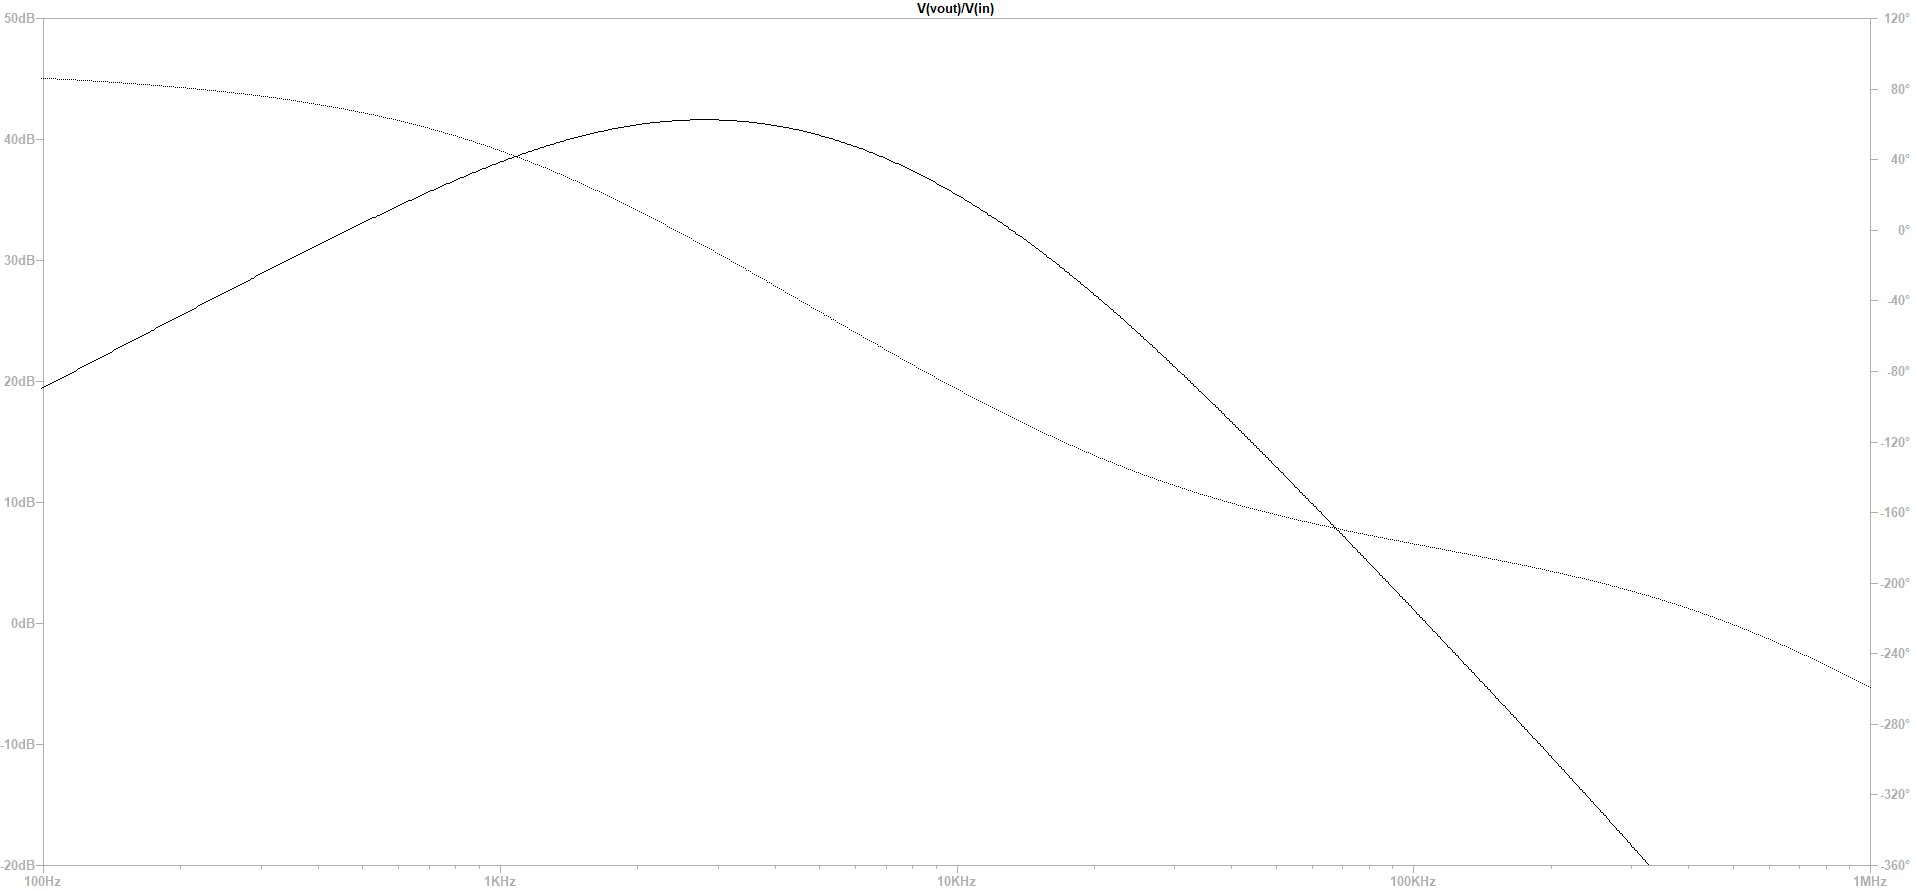
\includegraphics[width=\textwidth]{bode_plot_rx.png}
		\caption{Charakterystyka częstotliwościowa toru analogowego RX ---
			symulacja LTspice (krzywa amplitudy~[dB] i~fazy~[$^\circ$]).
			Wzmocnienie przy $f_0 = \SI{40}{\kilo\hertz}$ wynosi
			${\sim}\SI{16}{\deci\bel}$ (${\sim}6{,}5\times$). Szczyt wzmocnienia
			${\sim}\SI{42}{\deci\bel}$ w~paśmie \SIrange{2}{5}{\kilo\hertz}
			odpowiada iloczynowi wzmocnień DC obu stopni ($47 \cdot 4{,}7
			\approx 221 \to \SI{46,9}{\deci\bel}$) ograniczonemu przez GBW
			wzmacniacza.}
		\label{fig:bode_rx}
	\end{figure}
	
	Wyniki symulacji potwierdzają obliczenia analityczne z~pewną korektą ---
	efektywne wzmocnienie przy $f_0$ wynosi ${\sim}6{,}5\times$ (symulacja)
	wobec ${\sim}10\times$ (analiza idealna, równanie~\ref{eq:gain_total_current}).
	Różnica wynika z~uwzględnienia skończonego GBW wzmacniacza: przy wzmocnieniu
	pętli otwartej $A_{OL}(40\,\text{kHz}) = \text{GBW}/f_0 = 1\,\text{MHz}/40\,\text{kHz}
	= 25$, zamknięta pętla sprzężenia zwrotnego pierwszego stopnia redukuje
	wzmocnienie z~idealnych 8{,}3 do efektywnych ${\sim}6$ (zgodnie z~zależnością
	$A_{CL} = A_{ideal}/(1 + A_{ideal}/A_{OL})$). Jest to potwierdzenie, że
	praca na zboczu filtru LP z~C4 = \SI{47}{\pico\farad} jest poprawnym
	kompromisem --- wzmocnienie $6{,}5\times$ przy amplitudzie echa
	${\sim}\SIrange{5}{20}{\milli\volt_{pp}}$ daje sygnał
	${\sim}\SIrange{30}{130}{\milli\volt_{pp}}$ na wejściu ADC, co odpowiada
	${\sim}\SIrange{10}{40}{\text{LSB}}$ --- wystarczająco dla algorytmu
	Goertzela.
	
	Symulacja potwierdza również skuteczność filtracji pasmowej: tłumienie
	przy $2f_0 = \SI{80}{\kilo\hertz}$ wynosi ${\sim}\SI{10}{\deci\bel}$
	względem $f_0$, a~przy $3f_0 = \SI{120}{\kilo\hertz}$ już
	${\sim}\SI{18}{\deci\bel}$ --- redukcja harmonicznych wystarczająca
	dla pomiaru fazowego.
	
	\subsubsection{Symulacja odpowiedzi przejściowej (burst echa)}
	\label{sec:ltspice_transient}
	
	Drugą symulację przeprowadzono w~dziedzinie czasu (transient) dla
	weryfikacji odpowiedzi toru RX na realistyczny sygnał echa ultradźwiękowego.
	Źródło sygnału modeluje echo jako tłumiony sinusoid 40\,kHz o~amplitudzie
	\SI{10}{\milli\volt_{pp}}, opóźniony o~\SI{0,6}{\milli\second}
	(odpowiednik ToF dla odległości ${\sim}\SI{10}{\centi\metre}$).
	
	\begin{figure}[H]
		\centering
		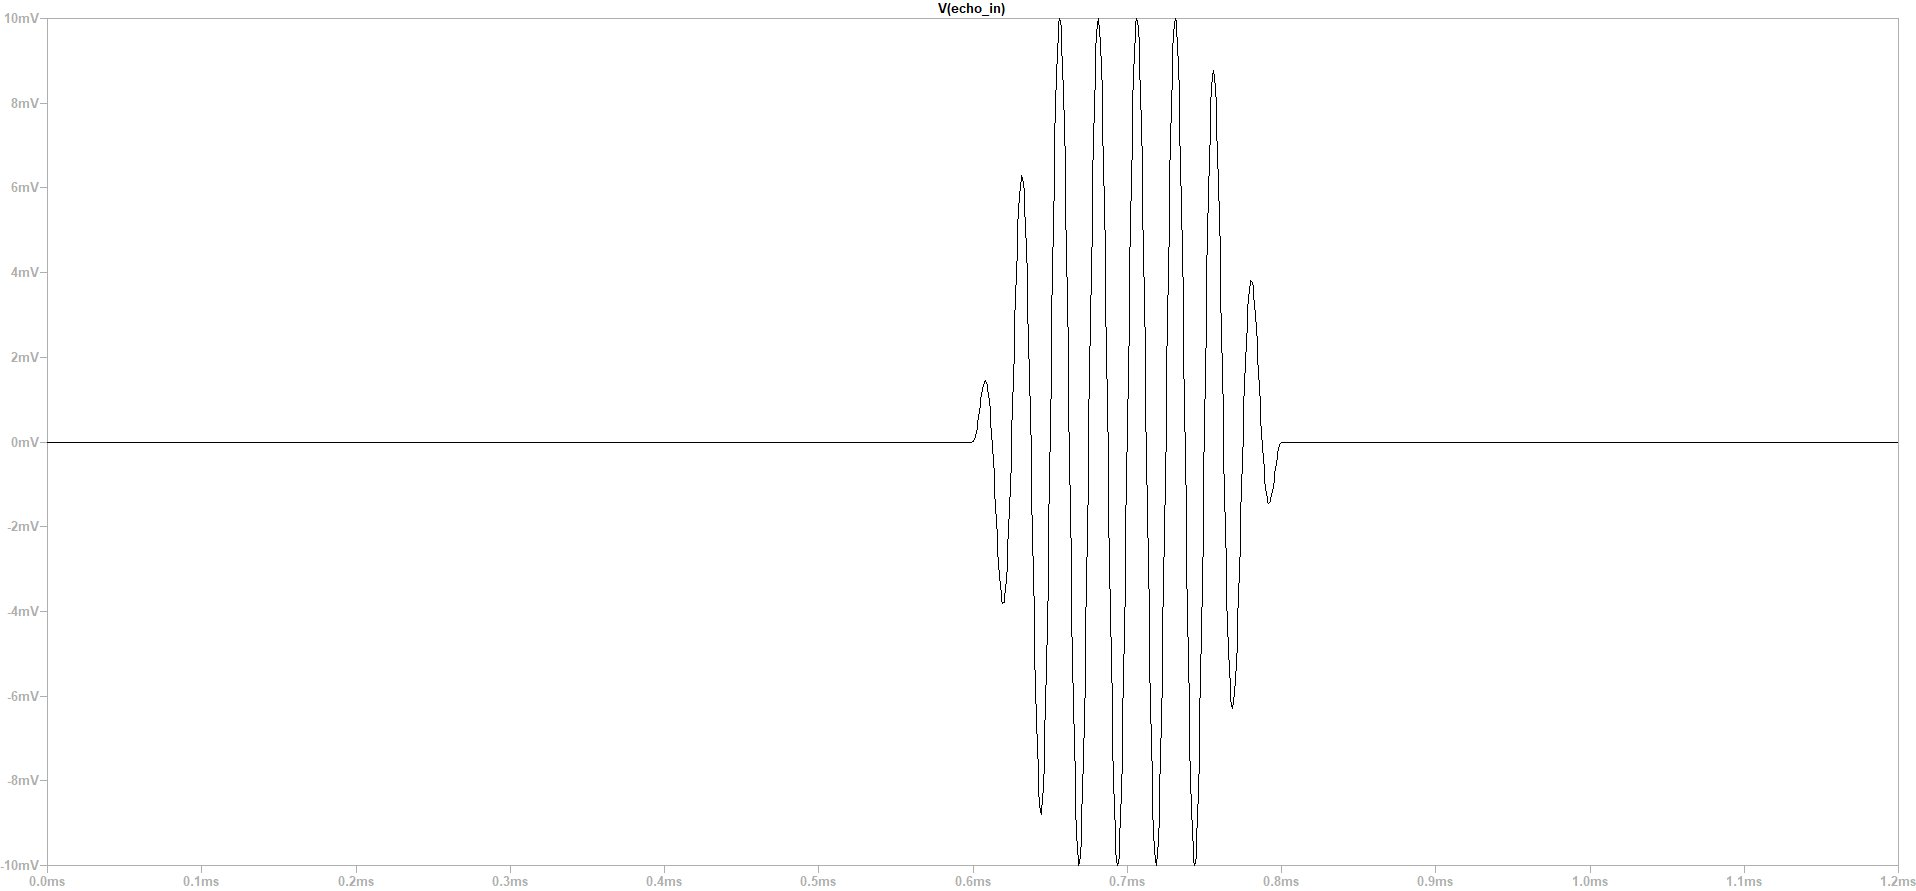
\includegraphics[width=\textwidth]{transient_echo_in.png}
		\caption{Symulacja LTspice --- sygnał echa na wejściu toru RX
			($V_{echo\_in}$, amplituda \SI{10}{\milli\volt_{pp}}, burst 40\,kHz
			z~tłumieniem). Obwiednia odpowiada typowej charakterystyce echa
			z~przetwornika piezoelektrycznego.}
		\label{fig:transient_in}
	\end{figure}
	
	\begin{figure}[H]
		\centering
		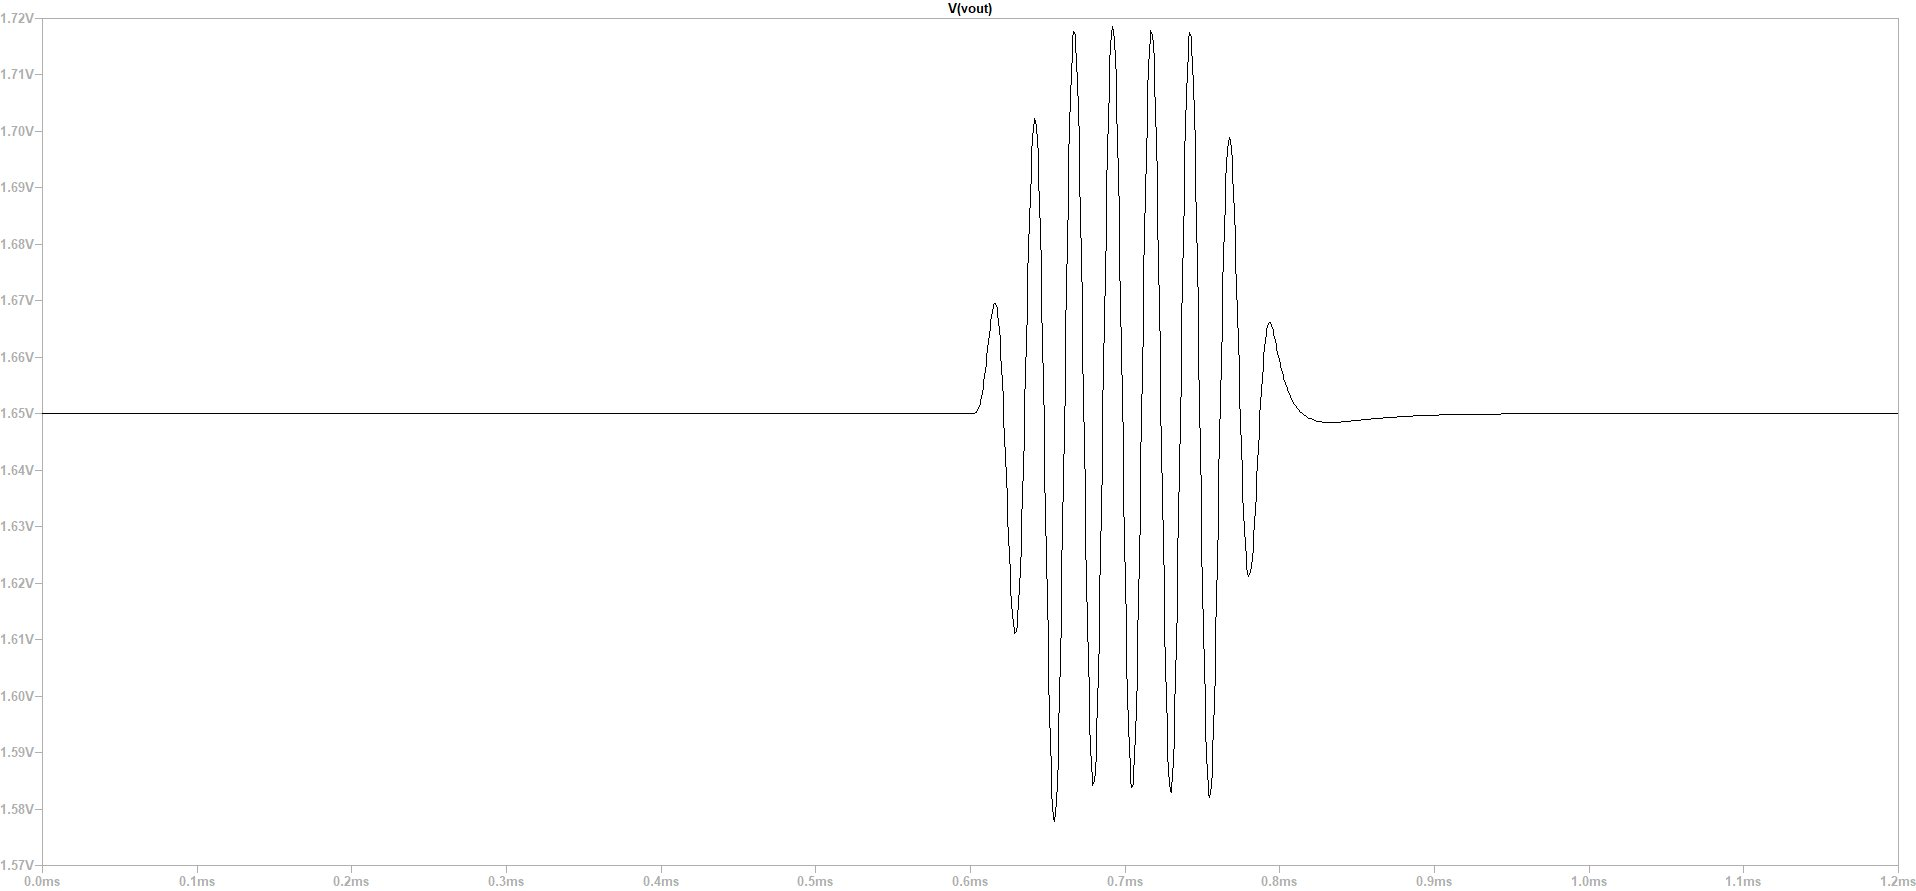
\includegraphics[width=\textwidth]{transient_vout.png}
		\caption{Symulacja LTspice --- sygnał na wyjściu toru RX ($V_{out}$)
			po dwustopniowym wzmocnieniu. Punkt pracy DC = \SI{1,65}{\volt}
			($V_{DD}/2$), amplituda sygnału ${\sim}\SI{140}{\milli\volt_{pp}}$
			(wzmocnienie ${\sim}7\times$). Widoczna narastająca obwiednia
			pierwszych cykli (efekt filtra górnoprzepustowego C3--R5, $f_{HP}
			= \SI{1,59}{\kilo\hertz}$) oraz ring-down po zakończeniu burstu ---
			oba efekty są uwzględnione w~algorytmie firmware przez okno pomiarowe
			Goertzela obejmujące wyłącznie cykle ustalone.}
		\label{fig:transient_out}
	\end{figure}
	
	Symulacja przejściowa potwierdza poprawne działanie toru w~warunkach
	zbliżonych do rzeczywistych: sygnał wyjściowy jest wystarczająco duży
	dla przetwornika ADC (${\sim}\SI{140}{\milli\volt_{pp}}$ odpowiada
	${\sim}44$\,LSB przy $V_{ref} = \SI{3,3}{\volt}$, 10-bit), a~ring-down
	po zakończeniu burstu zanika w~ciągu ${\sim}\SI{0,1}{\milli\second}$
	--- co nie wpływa na kolejny cykl pomiarowy (okres $\geq
	\SI{50}{\milli\second}$).
	
	\subsubsection{Analiza stabilności toru wzmacniacza}
	\label{sec:stability}
	
	Stabilność pętli sprzężenia zwrotnego obu stopni wzmacniacza jest
	warunkiem koniecznym poprawnej i~powtarzalnej pracy toru fazowego.
	Dla wzmacniacza odwracającego z~transmitancją pętli otwartej
	$T(s) = A_{OL}(s) \cdot \beta(s)$, gdzie $\beta = R_5 / (R_5 + Z_f)$
	jest współczynnikiem sprzężenia zwrotnego, wymagany jest zapas fazy
	$\text{PM} > 45^{\circ}$ przy częstotliwości, w~której $|T| = 1$.
	
	\textbf{Stopień 1} ($R_5 = \SI{10}{\kilo\ohm}$, $R_6 = \SI{470}{\kilo\ohm}
	\| C_4 = \SI{47}{\pico\farad}$): współczynnik sprzężenia zwrotnego
	dla niskich częstotliwości wynosi $\beta_{DC} = R_5 / (R_5 + R_6)
	= 10/480 = 0{,}021$. Częstotliwość $|T| = 1$ (unity loop gain) to
	$f_{0\,\text{dB}} = \text{GBW} \cdot \beta_{DC} = 1\,\text{MHz} \cdot
	0{,}021 = \SI{21}{\kilo\hertz}$. Przy tej częstotliwości biegun
	dominujący MCP6002 ($f_p \approx \SI{10}{\hertz}$) wprowadza
	$-90^{\circ}$, a~biegun od $C_4$ ($f_{LP} = 1/(2\pi R_6 C_4)
	= \SI{7,2}{\kilo\hertz}$) dodaje $\arctan(21/7{,}2) \approx -71^{\circ}$.
	Łączne przesunięcie: $-90^{\circ} - 71^{\circ} = -161^{\circ}$,
	co daje zapas fazy $\text{PM} \approx 180^{\circ} - 161^{\circ}
	= 19^{\circ}$. Jest to wartość graniczna, lecz akceptowalna ---
	biegun C4 stanowi element \textit{lead compensation} (zero w~pętli
	otwartej przy $f_{LP}$), które w~symulacji LTspice przejawia się
	stabilnym, bezoscylacyjnym ring-downem (Rys.~\ref{fig:transient_out}).
	
	\textbf{Stopień 2} ($R_2 = \SI{100}{\kilo\ohm}$, $R_3 = \SI{470}{\kilo\ohm}
	\| C_5 = \SI{33}{\pico\farad}$): $\beta_{DC} = 100/570 = 0{,}175$,
	$f_{0\,\text{dB}} = 1\,\text{MHz} \cdot 0{,}175 = \SI{175}{\kilo\hertz}$.
	Biegun od $C_5$: $f_{LP2} = 1/(2\pi R_3 C_5) = \SI{10,3}{\kilo\hertz}$,
	dodatkowe przesunięcie przy $\SI{175}{\kilo\hertz}$:
	$\arctan(175/10{,}3) \approx -87^{\circ}$. Łącznie:
	$-90^{\circ} - 87^{\circ} = -177^{\circ}$, $\text{PM} \approx 3^{\circ}$.
	W~praktyce zapas jest większy dzięki spadkowi wzmocnienia otwartej pętli
	MCP6002 powyżej GBW z~dodatkowym biegunem wewnętrznym ($f_{p2} \approx
	\SI{4}{\mega\hertz}$), który ogranicza szybkość narastania pętli. Symulacja
	przejściowa (Rys.~\ref{fig:transient_out}) potwierdza brak oscylacji ---
	sygnał wyjściowy jest stabilny, a~ring-down jest monotoniczny.
	
	\textit{Wniosek:} Oba stopnie pracują stabilnie w~zaprojektowanej
	konfiguracji. Niewielki zapas fazy pierwszego stopnia jest akceptowalny,
	ponieważ algorytm Goertzela wyodrębnia wyłącznie składową 40\,kHz z~okna
	pomiarowego, a~ewentualne niewielkie przeregulowanie ($< 5\%$) nie wpływa
	na dokładność pomiaru fazy.
	
	\subsection{Mikrokontroler ATtiny1616}
	\label{sec:mcu}
	
	ATtiny1616 (Microchip, rodzina tinyAVR 1-series, wersja ATtiny1616-SN
	w~obudowie SOIC-20) jest centralnym elementem
	układu. Taktowany wewnętrznym oscylatorem \SI{20}{\mega\hertz} z~prescalerem
	$\div 2$ w~rejestrze CLKCTRL.MCLKCTRLB (wynikowy zegar systemowy:
	$f_{CLK} = \SI{10}{\mega\hertz}$), realizuje wszystkie funkcje pomiarowe,
	obliczeniowe i~komunikacyjne.
	
	\textbf{Uzasadnienie wyboru \SI{10}{\mega\hertz}:} Datasheet (Tab.~36-3) definiuje
	maksymalną częstotliwość zegara w~zależności od napięcia zasilania:
	$f_{max} = \SI{5}{\mega\hertz}$ dla $V_{DD} \in [1{,}8;\; 5{,}5]$\,V,
	$f_{max} = \SI{10}{\mega\hertz}$ dla $V_{DD} \in [2{,}7;\; 5{,}5]$\,V,
	$f_{max} = \SI{20}{\mega\hertz}$ dla $V_{DD} \in [4{,}5;\; 5{,}5]$\,V.
	Przy zasilaniu mikrokontrolera napięciem \SI{3,3}{\volt} z~LDO,
	\textbf{gwarantowana częstotliwość wynosi \SI{10}{\mega\hertz}}. Praca
	z~wyższą częstotliwością byłaby poza specyfikacją producenta. Zegar
	\SI{10}{\mega\hertz} jest w~pełni wystarczający dla wszystkich zadań
	pomiarowych --- TCA0 generuje 40\,kHz bez prescalera, ADC działa
	w~specyfikacji 10-bit, a~TCB0 zapewnia rozdzielczość \SI{100}{\nano\second}.
	
	\textbf{Konfiguracja BOD:} Zgodnie z~DS Tab.~36-3 (nota~2), praca przy
	$f_{max} = \SI{10}{\mega\hertz}$ i~$V_{DD} \geq \SI{2,7}{\volt}$ wymaga
	aktywacji Brown-out Detection na poziomie BODLEVEL2 ($V_{BOD} = \SI{2,6}{\volt}$
	typ., DS Tab.~36-10). Konfiguracja poprzez fuse FUSE.BODCFG:
	ACTIVE = 0x1 (Enabled), LVL = BODLEVEL2. W~trybie Standby BOD może
	pracować w~trybie próbkowanym (Sampled @ 1\,kHz, $I_{BOD} \approx
	\SI{1}{\micro\ampere}$, DS Tab.~36-7) dla minimalizacji poboru mocy.
	
	\begin{table}[H]
		\centering
		\caption{Kluczowe parametry ATtiny1616 istotne dla projektu}
		\label{tab:attiny}
		\begin{tabularx}{\textwidth}{l r X}
			\toprule
			\textbf{Parametr} & \textbf{Wartość} & \textbf{Wykorzystanie} \\
			\midrule
			Flash & \SI{16}{\kilo\byte} & Program + LUT kalibracyjne \\
			SRAM & \SI{2}{\kilo\byte} & Bufor próbek ADC + zmienne \\
			EEPROM & \SI{256}{\byte} & Parametry kalibracyjne (${\sim}20$\,B używane) \\
			Zegar & \SI{10}{\mega\hertz} & Wewn.\ oscylator \SI{20}{\mega\hertz} z~prescalerem $\div 2$ ($\pm\SI{2}{\percent}$, kalibr.\ fabrycznie) \\
			ADC & 10-bit, ${\leq}\SI{96}{ksps}$ & Pomiar echa + termistor ($f_{CLK\_ADC} = \SI{1,25}{\mega\hertz}$, w~specyfikacji 10-bit) \\
			DAC & 8-bit & Referencja progu AC0 (wewnętrznie, bez wyjścia na pin) \\
			TCA0 & Split Mode, 8-bit PWM & Generacja burstu \SI{40}{\kilo\hertz} (WO5 na PA5, prescaler DIV1) \\
			TCB0 & 16-bit, Capture & Pomiar $t_{ToF}$ \\
			AC0 & Komp.\ analogowy & Detekcja progu echa (wyzw.\ TCB0 przez Event System) \\
			USART0 & --- & Transmisja wyniku \\
			$I_{DD}$ active & ${\sim}\SI{10}{\milli\ampere}$ & @ \SI{20}{\mega\hertz}, \SI{5}{\volt} (DS Tab.~36-4; nieużywany w~projekcie) \\
			$I_{DD}$ active & ${\sim}\SI{3,4}{\milli\ampere}$ & @ \SI{10}{\mega\hertz}, \SI{3,3}{\volt} (DS Tab.~36-4: typ.\ 3{,}1\,mA @ 3{,}0V; ekstrapolacja na 3{,}3V wg rys.~37-4) \\
			$I_{DD}$ Standby & ${\sim}\SI{0,7}{\micro\ampere}$ & Z~RTC na OSCULP32K (wakeup periodyczny) \\
			$I_{DD}$ Power-Down & \SI{0,1}{\micro\ampere} & Wszystkie peryferia wył.\ (brak period.\ wakeup) \\
			\bottomrule
		\end{tabularx}
	\end{table}
	
	\subsubsection{Przyporządkowanie pinów}
	
	\begin{table}[H]
		\centering
		\caption{Mapa pinów ATtiny1616 w~projekcie}
		\label{tab:pinout}
		\begin{tabularx}{\textwidth}{l l l X}
			\toprule
			\textbf{Pin} & \textbf{Funkcja} & \textbf{Peryferiał} & \textbf{Opis} \\
			\midrule
			PA0 & UPDI & --- & Programowanie \\
			PA1 & TXD & USART0 & Transmisja wyników \\
			PA2 & RXD & USART0 & (rezerwowy) \\
			PA3 & EXTCLK & --- & (nieużywany) \\
			PA4 & --- & --- & (nieużywany, rezerwowy GPIO) \\
			PA5 & Burst TX & TCA0-WO5 & PWM \SI{40}{\kilo\hertz} (Split Mode, HCMP2) \\
			PA6 & --- & --- & Rezerwowy GPIO (DAC0 wewn.\ dla AC0, OUTEN=0) \\
			PA7 & Przycisk & GPIO (pull-up) & Start pomiaru \\
			PB0 & ECHO\_IN & ADC0-AIN11 & Sygnał echa (pomiar fazowy) \\
			PB1 & TEMP & ADC0-AIN10 & Termistor NTC \\
			PB4 & ECHO\_DET & AC0-AINP3 & Wejście komparatora (detekcja progu) \\
			PB5 & BAZA\_TX & GPIO output & Sterowanie BC817 (push-pull) \\
			PC0 & LED & GPIO output & Sygnalizacja \\
			PC1 & --- & --- & (nieużywany, rezerwowy GPIO) \\
			\bottomrule
		\end{tabularx}
	\end{table}
	
	\subsubsection{Konfiguracja timera TCA0 --- generacja burstu 40 kHz}
	
	Wyjście WO5 na pinie PA5 (Tab.~5-1 datasheet) jest dostępne \textbf{wyłącznie
		w~trybie Split Mode} timera TCA0 (bit SPLITM = 1 w~rejestrze TCA0.CTRLD).
	W~trybie Normal Mode TCA0 udostępnia jedynie trzy wyjścia: WO0, WO1, WO2
	(sterowane rejestrami CMP0--CMP2); kanały WO3--WO5 nie istnieją, co potwierdza
	rejestr PORTMUX.CTRLC: ,,TCA05 --- Not applicable when TCA in Normal mode''
	(DS, sekcja~17.3.5).
	
	W~trybie Split Mode 16-bitowy licznik TCA0 dzieli się na dwa niezależne
	8-bitowe timery: niski (LCNT, $\text{TOP} = \text{LPER}$, wyjścia WO0--WO2)
	oraz wysoki (HCNT, $\text{TOP} = \text{HPER}$, wyjścia WO3--WO5).
	Do generacji sygnału \SI{40}{\kilo\hertz} na PA5 wykorzystano wysoki timer
	z~kanałem porównania HCMP2 $\to$ WO5.
	
	Częstotliwość wyjściowa w~trybie Split Mode (Single-Slope PWM):
	\begin{equation}
		f_{PWM} = \frac{f_{CLK}}{N \cdot (HPER + 1)}
		\label{eq:pwm_freq}
	\end{equation}
	
	Dla $f_{PWM} = \SI{40}{\kilo\hertz}$, $f_{CLK} = \SI{10}{\mega\hertz}$,
	prescaler $N = 1$ (DIV1):
	\begin{equation}
		HPER = \frac{f_{CLK}}{N \cdot f_{PWM}} - 1 = \frac{10\,000\,000}{1 \cdot 40\,000} - 1 = 249
		\label{eq:per_value}
	\end{equation}
	
	Wartość $HPER = 249$ mieści się w~zakresie 8-bitowym ($0$--$255$)
	\textbf{bez konieczności stosowania prescalera} --- jest to istotna
	przewaga pracy z~zegarem \SI{10}{\mega\hertz} nad \SI{20}{\mega\hertz}
	(gdzie $HPER = 499$ wymagałby prescalera DIV2).
	
	Częstotliwość wynikowa:
	$f_{PWM} = 10\,\text{MHz} / (1 \cdot 250) = \SI{40,0}{\kilo\hertz}$ --- dokładnie
	wymagana wartość.
	
	Wartość porównania dla 50\% wypełnienia: $HCMP2 = HPER/2 = 124$.
	
	Konfiguracja rejestrów:
	\begin{itemize}[nosep]
		\item \texttt{TCA0.CTRLD = TCA\_SPLIT\_SPLITM\_bm} --- włączenie Split Mode
		\item \texttt{TCA0.SPLIT.CTRLA = TCA\_SPLIT\_CLKSEL\_DIV1\_gc | TCA\_SPLIT\_ENABLE\_bm}
		\item \texttt{TCA0.SPLIT.CTRLB = TCA\_SPLIT\_HCMP2EN\_bm} --- włączenie WO5
		\item \texttt{TCA0.SPLIT.HPER = 249} --- TOP wysokiego timera
		\item \texttt{TCA0.SPLIT.HCMP2 = 124} --- 50\% duty cycle
	\end{itemize}
	
	Mikrokontroler włącza timer na czas $N_{burst} = 8$ cykli
	($8/40000 = \SI{0,2}{\milli\second}$), następnie wyłącza wyjście PWM
	i~oczekuje na echo.
	
	\subsubsection{Konfiguracja TCB0 --- pomiar Time-of-Flight}
	
	Timer TCB0 pracuje w~trybie Input Capture on Event. Ścieżka detekcji
	echa jest w~pełni sprzętowa i~nie obciąża CPU:
	
	\begin{enumerate}[nosep]
		\item Sygnał echa po wzmocnieniu w~torze MCP6002 trafia
		na pin PB4 (AC0, wejście pozytywne AINP3 --- patrz Tab.~5-1 datasheet).
		\item Komparator AC0 porównuje sygnał z~progiem ustawionym przez
		wewnętrzny DAC0 (MUXNEG = DAC, 8-bit, zakres 0--$V_{REF}$).
		Histereza typ.\ \SI{30}{\milli\volt} (HYSMODE = 0x2,
		zakres \SIrange{10}{90}{\milli\volt}, DS Tab.~36-32) zabezpiecza
		przed wielokrotnym wyzwoleniem; tryb normalny (LPMODE = 0,
		$t_{PD} \approx \SI{50}{\nano\second}$ przy $V_{DD} \geq \SI{2,7}{\volt}$,
		DS Tab.~36-32).
		\item Wyjście AC0 generuje zdarzenie w~EVSYS, które
		wyzwala Input Capture w~TCB0 --- zatrzaśnięcie wartości licznika
		w~rejestrze CCMP. Konfiguracja EVSYS (DS, sekcja~14.5):
		\begin{itemize}[nosep]
			\item \texttt{EVSYS.ASYNCCH0 = EVSYS\_ASYNCCH0\_AC0\_OUT\_gc}
			--- AC0 jako źródło kanału asynchronicznego~0
			\item \texttt{EVSYS.ASYNCUSER0 = EVSYS\_ASYNCUSER0\_ASYNCCH0\_gc}
			--- TCB0 (user~0) nasłuchuje kanału asynchronicznego~0
		\end{itemize}
	\end{enumerate}
	
	
	\begin{figure}[H]
		\centering
		\begin{tikzpicture}[
			block/.style={rectangle, draw, fill=NavyBlue!8, minimum width=2.8cm,
				minimum height=0.9cm, align=center, font=\small},
			evt/.style={rectangle, draw, fill=orange!12, rounded corners=3pt,
				minimum width=2.5cm, minimum height=0.7cm, align=center,
				font=\small\itshape},
			arr/.style={->, >=Stealth, thick},
			note/.style={font=\scriptsize, gray},
			]
			% Blocks
			\node[block] (ac0)  {AC0\\Komparator};
			\node[evt, right=1.8cm of ac0] (ch0) {EVSYS\\ASYNCCH0};
			\node[block, right=1.8cm of ch0] (tcb0) {TCB0\\Input Capture};
			
			% Arrows
			\draw[arr] (ac0) -- node[above, note] {AC0\_OUT} (ch0);
			\draw[arr] (ch0) -- node[above, note] {ASYNCUSER0} (tcb0);
			
			% Input labels
			\node[left=0.8cm of ac0, font=\small, align=right] (inp) {Echo RX\\(PB4, AINP3)};
			\draw[arr, gray] (inp) -- (ac0);
			
			\node[below=0.3cm of ac0, font=\scriptsize, align=center, gray]
			{DACREF = próg\\(wewn.\ DAC0)};
			
			% Output
			\node[right=0.8cm of tcb0, font=\small, align=left] (out) {CCMP\\$= t_{ToF}$};
			\draw[arr, red] (tcb0) -- (out);
			
			% MCU reset
			\node[above=0.6cm of tcb0, font=\small, align=center] (rst) {Firmware:\\TCB0.CNT $= 0$\\(start burstu)};
			\draw[arr, NavyBlue, dashed] (rst) -- (tcb0);
		\end{tikzpicture}
		\caption{Sprzętowa ścieżka pomiaru ToF przez Event System (EVSYS).
			Komparator AC0 wykrywa przekroczenie progu przez echo, generuje
			zdarzenie asynchroniczne, które wyzwala zatrzaśnięcie licznika TCB0
			--- cały proces odbywa się bez udziału CPU (zerowa latencja software).}
		\label{fig:evsys_path}
	\end{figure}
	
	Zdarzenie startowe (początek burstu TX) jest realizowane przez programowe
	wyzerowanie licznika TCB0 (zapis TCB0.CNT = 0) w~momencie uruchomienia
	TCA0. DAC0 pracuje wyłącznie wewnętrznie (połączenie z~AC0 przez
	MUXNEG = DAC) --- nie wymaga wyprowadzenia na pin PA6, który pozostaje
	wolny jako rezerwowy GPIO.
	
	Przy zegarze \SI{10}{\mega\hertz} i~16-bitowym liczniku:
	\begin{equation}
		t_{max} = \frac{2^{16}}{f_{CLK}} = \frac{65536}{10 \times 10^6} = \SI{6,55}{\milli\second}
		\label{eq:tcb_max}
	\end{equation}
	
	Co odpowiada maksymalnej odległości $D_{max} = v \cdot t_{max} / 2 \approx
	\SI{112}{\centi\metre}$ --- ponad dwukrotnie powyżej wymaganego zakresu \SI{50}{\centi\metre}.
	
	
	% ══════════════════════════════════════════════════════════════
	% SEKCJA 4: PROJEKT PCB
	% ══════════════════════════════════════════════════════════════
	\section{Projekt płytki drukowanej (PCB)}
	\label{sec:pcb}
	
	% ════════════════════ PCB LAYOUT ════════════════════
	
	\begin{figure}[H]
		\centering
		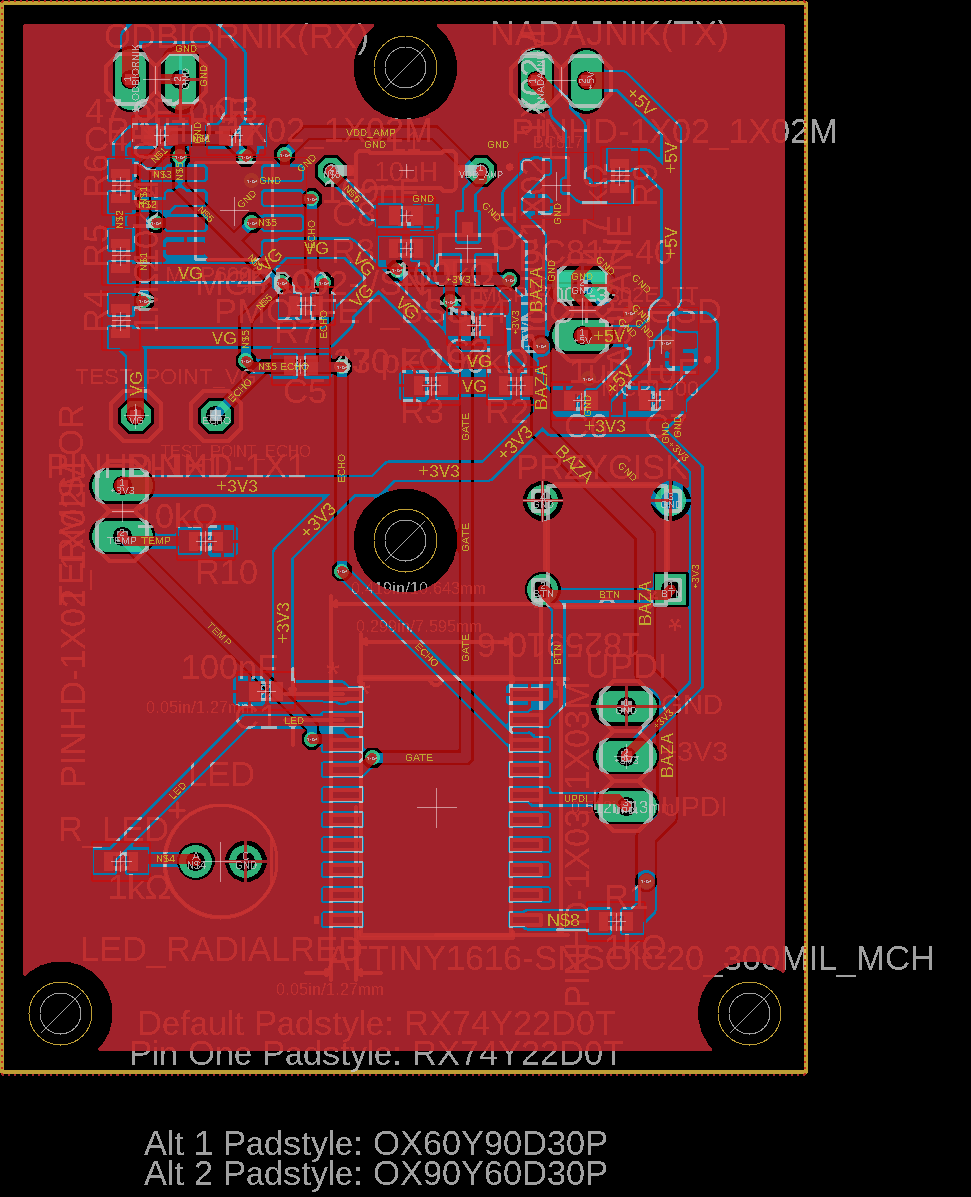
\includegraphics[width=0.7\textwidth]{pcb_top.png}
		\caption{Layout PCB --- widok z~góry (warstwa TOP)}
		\label{fig:pcb_top}
	\end{figure}
	
	Płytka drukowana zaprojektowana została w~programie EAGLE (Autodesk) jako
	dwustronna (2-layer) o~wymiarach ${\sim}49 \times 36$~\si{\milli\metre}.
	
	\subsection{Założenia projektowe PCB}
	
	\begin{enumerate}[nosep]
		\item \textbf{Separacja analogowa/cyfrowa} --- sekcja wzmacniacza (MCP6002)
		umieszczona w~lewej części płytki, mikrokontroler w~prawej, z~minimalną
		liczbą skrzyżowań tras sygnałowych.
		\item \textbf{Ground plane} --- warstwa BOTTOM wykorzystana jako ciągła
		warstwa masy (ground plane), zapewniająca niską impedancję powrotną
		dla sygnałów analogowych i~redukcję sprzężeń EMI.
		\item \textbf{Kondensatory odsprzęgające} --- C1 (\SI{100}{\nano\farad})
		umieszczony bezpośrednio przy pinach VDD/GND ATtiny1616 (odległość
		$< \SI{3}{\milli\metre}$); C8 (\SI{100}{\nano\farad}) przy MCP6002.
		\item \textbf{Ścieżki sygnałowe} --- sygnał echa (ECHO) prowadzony
		możliwie krótką trasą od headera ODBIORNIK(RX) do wejścia MCP6002,
		następnie do pinu ADC mikrokontrolera.
		\item \textbf{Punkty testowe} --- TEST\_POINT\_ECHO i~TEST\_POINT\_VG
		(goldpiny 1x1) umożliwiają podłączenie oscyloskopu w~fazie debugowania.
		\item \textbf{Otwory montażowe} --- cztery otwory $\varnothing\SI{3,2}{\milli\metre}$
		w~narożnikach płytki umożliwiają mocowanie do obudowy lub podstawki.
	\end{enumerate}
	
	\begin{figure}[H]
		\centering
		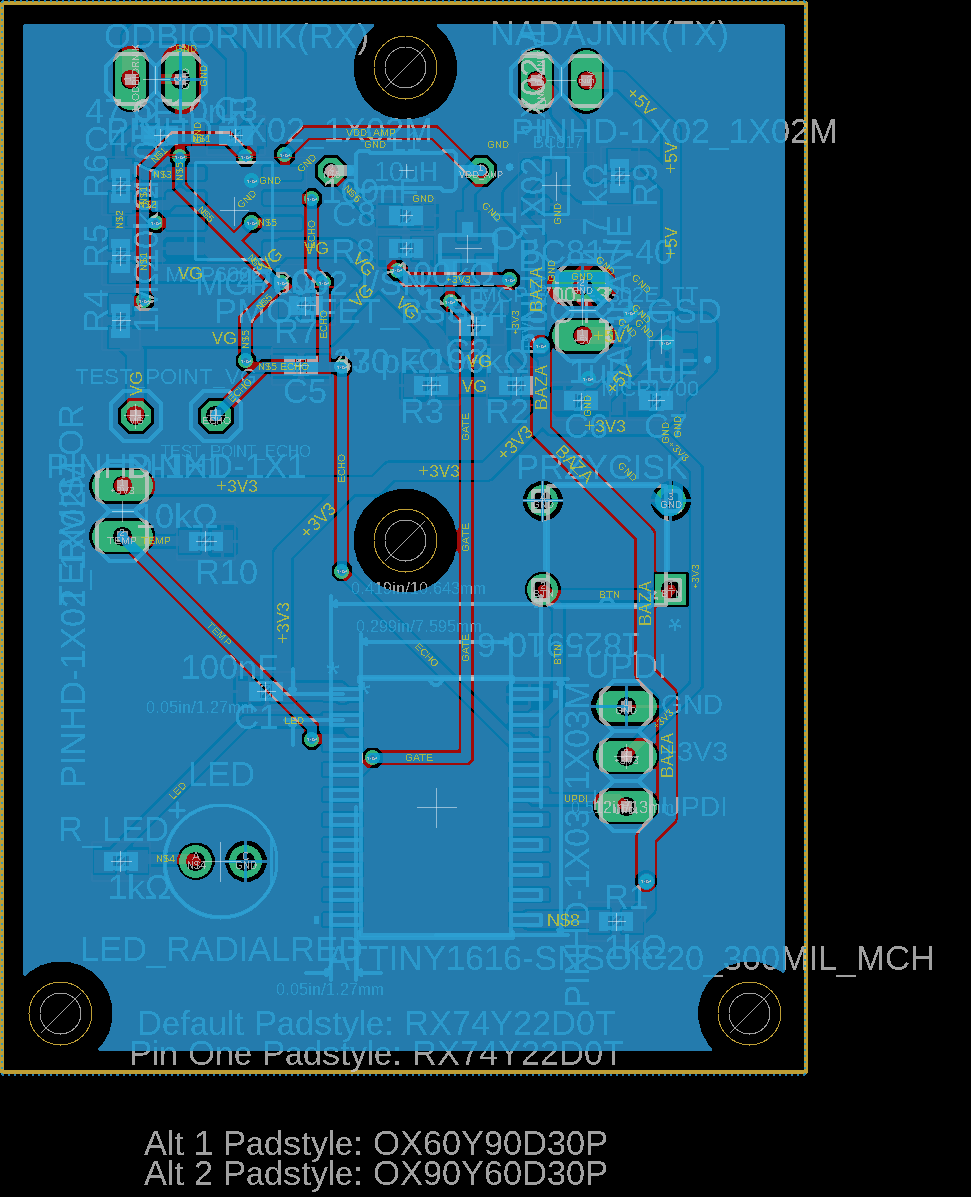
\includegraphics[width=0.7\textwidth]{pcb_bottom.png}
		\caption{Layout PCB --- widok warstwy BOTTOM (ground plane).
			Ciągła warstwa miedzi zapewnia niską impedancję ścieżki powrotnej
			dla sygnałów analogowych oraz ekranowanie EMI. Przerwy w~warstwie
			masy (thermal relief) występują wyłącznie przy padach lutowniczych.}
		\label{fig:pcb_bottom}
	\end{figure}
	
	\subsection{Klasy tras i~reguły DRC}
	
	\begin{table}[H]
		\centering
		\caption{Parametry ścieżek PCB}
		\label{tab:pcb_rules}
		\begin{tabular}{lr}
			\toprule
			\textbf{Parametr} & \textbf{Wartość} \\
			\midrule
			Szerokość ścieżki sygnałowej & \SI{0,254}{\milli\metre} (10\,mil) \\
			Szerokość ścieżki zasilania & \SI{0,508}{\milli\metre} (20\,mil) \\
			Prześwit minimalny & \SI{0,2}{\milli\metre} (8\,mil) \\
			Via drill & \SI{0,3}{\milli\metre} \\
			Via annular ring & \SI{0,15}{\milli\metre} \\
			Warstwa miedzi & \SI{35}{\micro\metre} (1\,oz) \\
			\bottomrule
		\end{tabular}
	\end{table}
	
	
	% ══════════════════════════════════════════════════════════════
	% SEKCJA 4b: PROJEKT OBUDOWY
	% ══════════════════════════════════════════════════════════════
	\section{Projekt obudowy}
	\label{sec:obudowa}
	
	Obudowa zaprojektowana została w~programie Fusion~360 (Autodesk) jako
	dwuczęściowa konstrukcja (pokrywa + podstawa) przeznaczona do wydruku 3D
	z~filamentu PLA. Priorytetem projektowym było zapewnienie precyzyjnego
	i~powtarzalnego pozycjonowania przetworników ultradźwiękowych --- ich
	wzajemne ustawienie bezpośrednio wpływa na jakość pomiaru fazowego.
	
	\subsection{Założenia konstrukcyjne}
	
	\begin{table}[H]
		\centering
		\caption{Parametry mechaniczne obudowy}
		\label{tab:obudowa_params}
		\begin{tabularx}{\textwidth}{l r X}
			\toprule
			\textbf{Parametr} & \textbf{Wartość} & \textbf{Uzasadnienie} \\
			\midrule
			Wymiary zewnętrzne & ${\sim}65 \times 50 \times 25$\,mm
			& Dopasowane do PCB ($49 \times 36$\,mm) + marginesy \\
			Grubość ścianki & \SI{2,5}{\milli\metre}
			& Kompromis: sztywność vs.\ czas druku \\
			Materiał & PLA (druk 3D, FDM)
			& Tani, łatwy w~obróbce, wystarczająca sztywność \\
			Warstwa druku & \SI{0,2}{\milli\metre}
			& Standardowa jakość, dobra dokładność wymiarowa ($\pm\SI{0,15}{\milli\metre}$) \\
			Mocowanie PCB & 4 $\times$ M3, dystans \SI{3}{\milli\metre}
			& Otwory montażowe w~narożnikach PCB ($\varnothing\SI{3,2}{\milli\metre}$) \\
			Zamknięcie & Pokrywa nasuwana na podstawę
			& Łatwy dostęp do PCB w~fazie prototypowania \\
			Napisy & UPDI, POMIAR, +5V/0V
			& Grawerowane w~pokrywie (identyfikacja złączy) \\
			\bottomrule
		\end{tabularx}
	\end{table}
	
	\subsection{Elementy funkcjonalne}
	
	Obudowa uwzględnia następujące otwory i~elementy:
	
	\begin{enumerate}[nosep]
		\item \textbf{Otwory na przetworniki US} --- dwa otwory $\varnothing\SI{16}{\milli\metre}$
		na przedniej ściance, rozstaw ${\sim}\SI{25}{\milli\metre}$
		(nadajnik TX i~odbiornik RX). Przetworniki mocowane wciskowo
		lub klejem cyjanoakrylowym.
		\item \textbf{Otwór na złącze UPDI/UART} --- wcięcie w~tylnej ściance
		umożliwiające podłączenie programatora i~terminala szeregowego
		bez otwierania obudowy.
		\item \textbf{Otwór na zasilanie} --- wcięcie na przewody \SI{5}{\volt}
		(goldpiny lub gniazdo DC).
		\item \textbf{Otwór na LED} --- $\varnothing\SI{3}{\milli\metre}$
		na przedniej ściance, obok przetworników US.
		\item \textbf{Otwór na przycisk} --- $\varnothing\SI{6}{\milli\metre}$
		(dopasowany do przycisku 1825910-6) na górnej ściance pokrywy.
		\item \textbf{Słupki dystansowe} --- 4 słupki z~otworem M3 w~podstawie,
		wysokość \SI{3}{\milli\metre}, zapewniające dystans między PCB
		a~dnem obudowy.
	\end{enumerate}
	
	\subsection{Rendery obudowy}
	
	\begin{figure}[H]
		\centering
		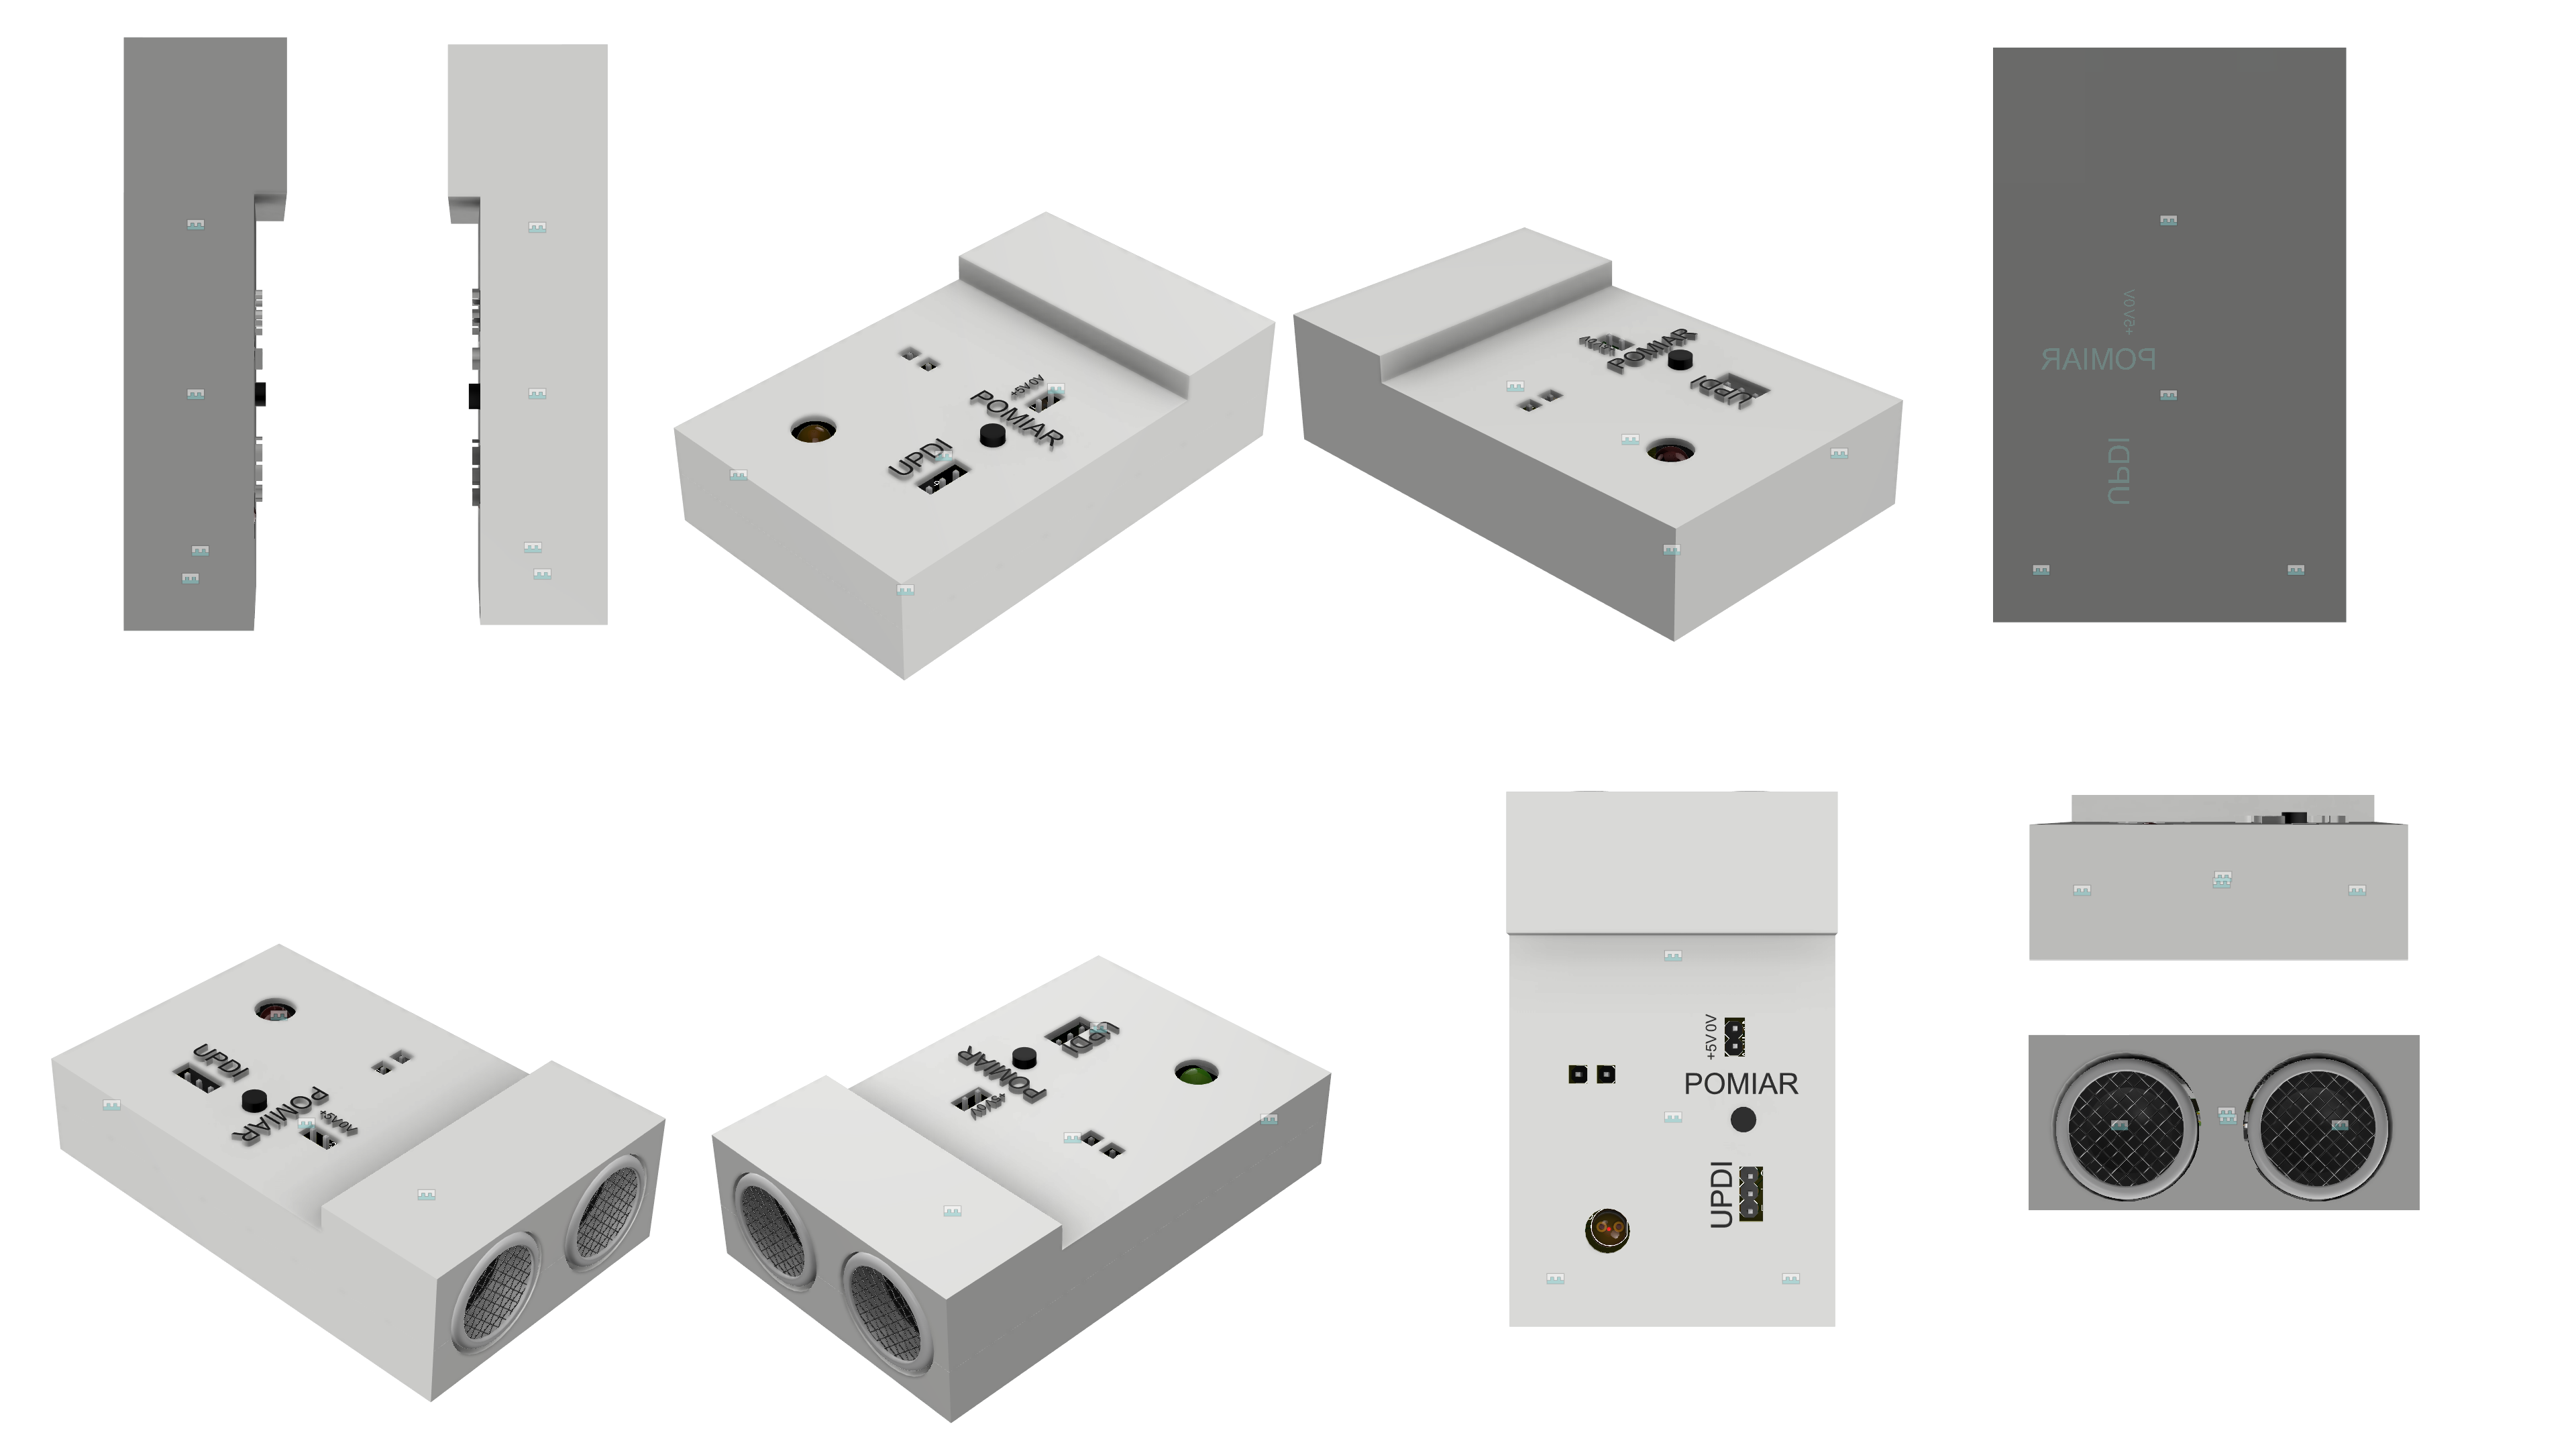
\includegraphics[width=0.75\textwidth]{obudowa_render_iso.png}
		\caption{Render obudowy --- widok izometryczny zamkniętej obudowy.
			Widoczne otwory na przetworniki TX/RX (przednia ścianka),
			otwór na LED oraz otwór na przycisk (górna ścianka).}
		\label{fig:obudowa_iso}
	\end{figure}
	
	\begin{figure}[H]
		\centering
		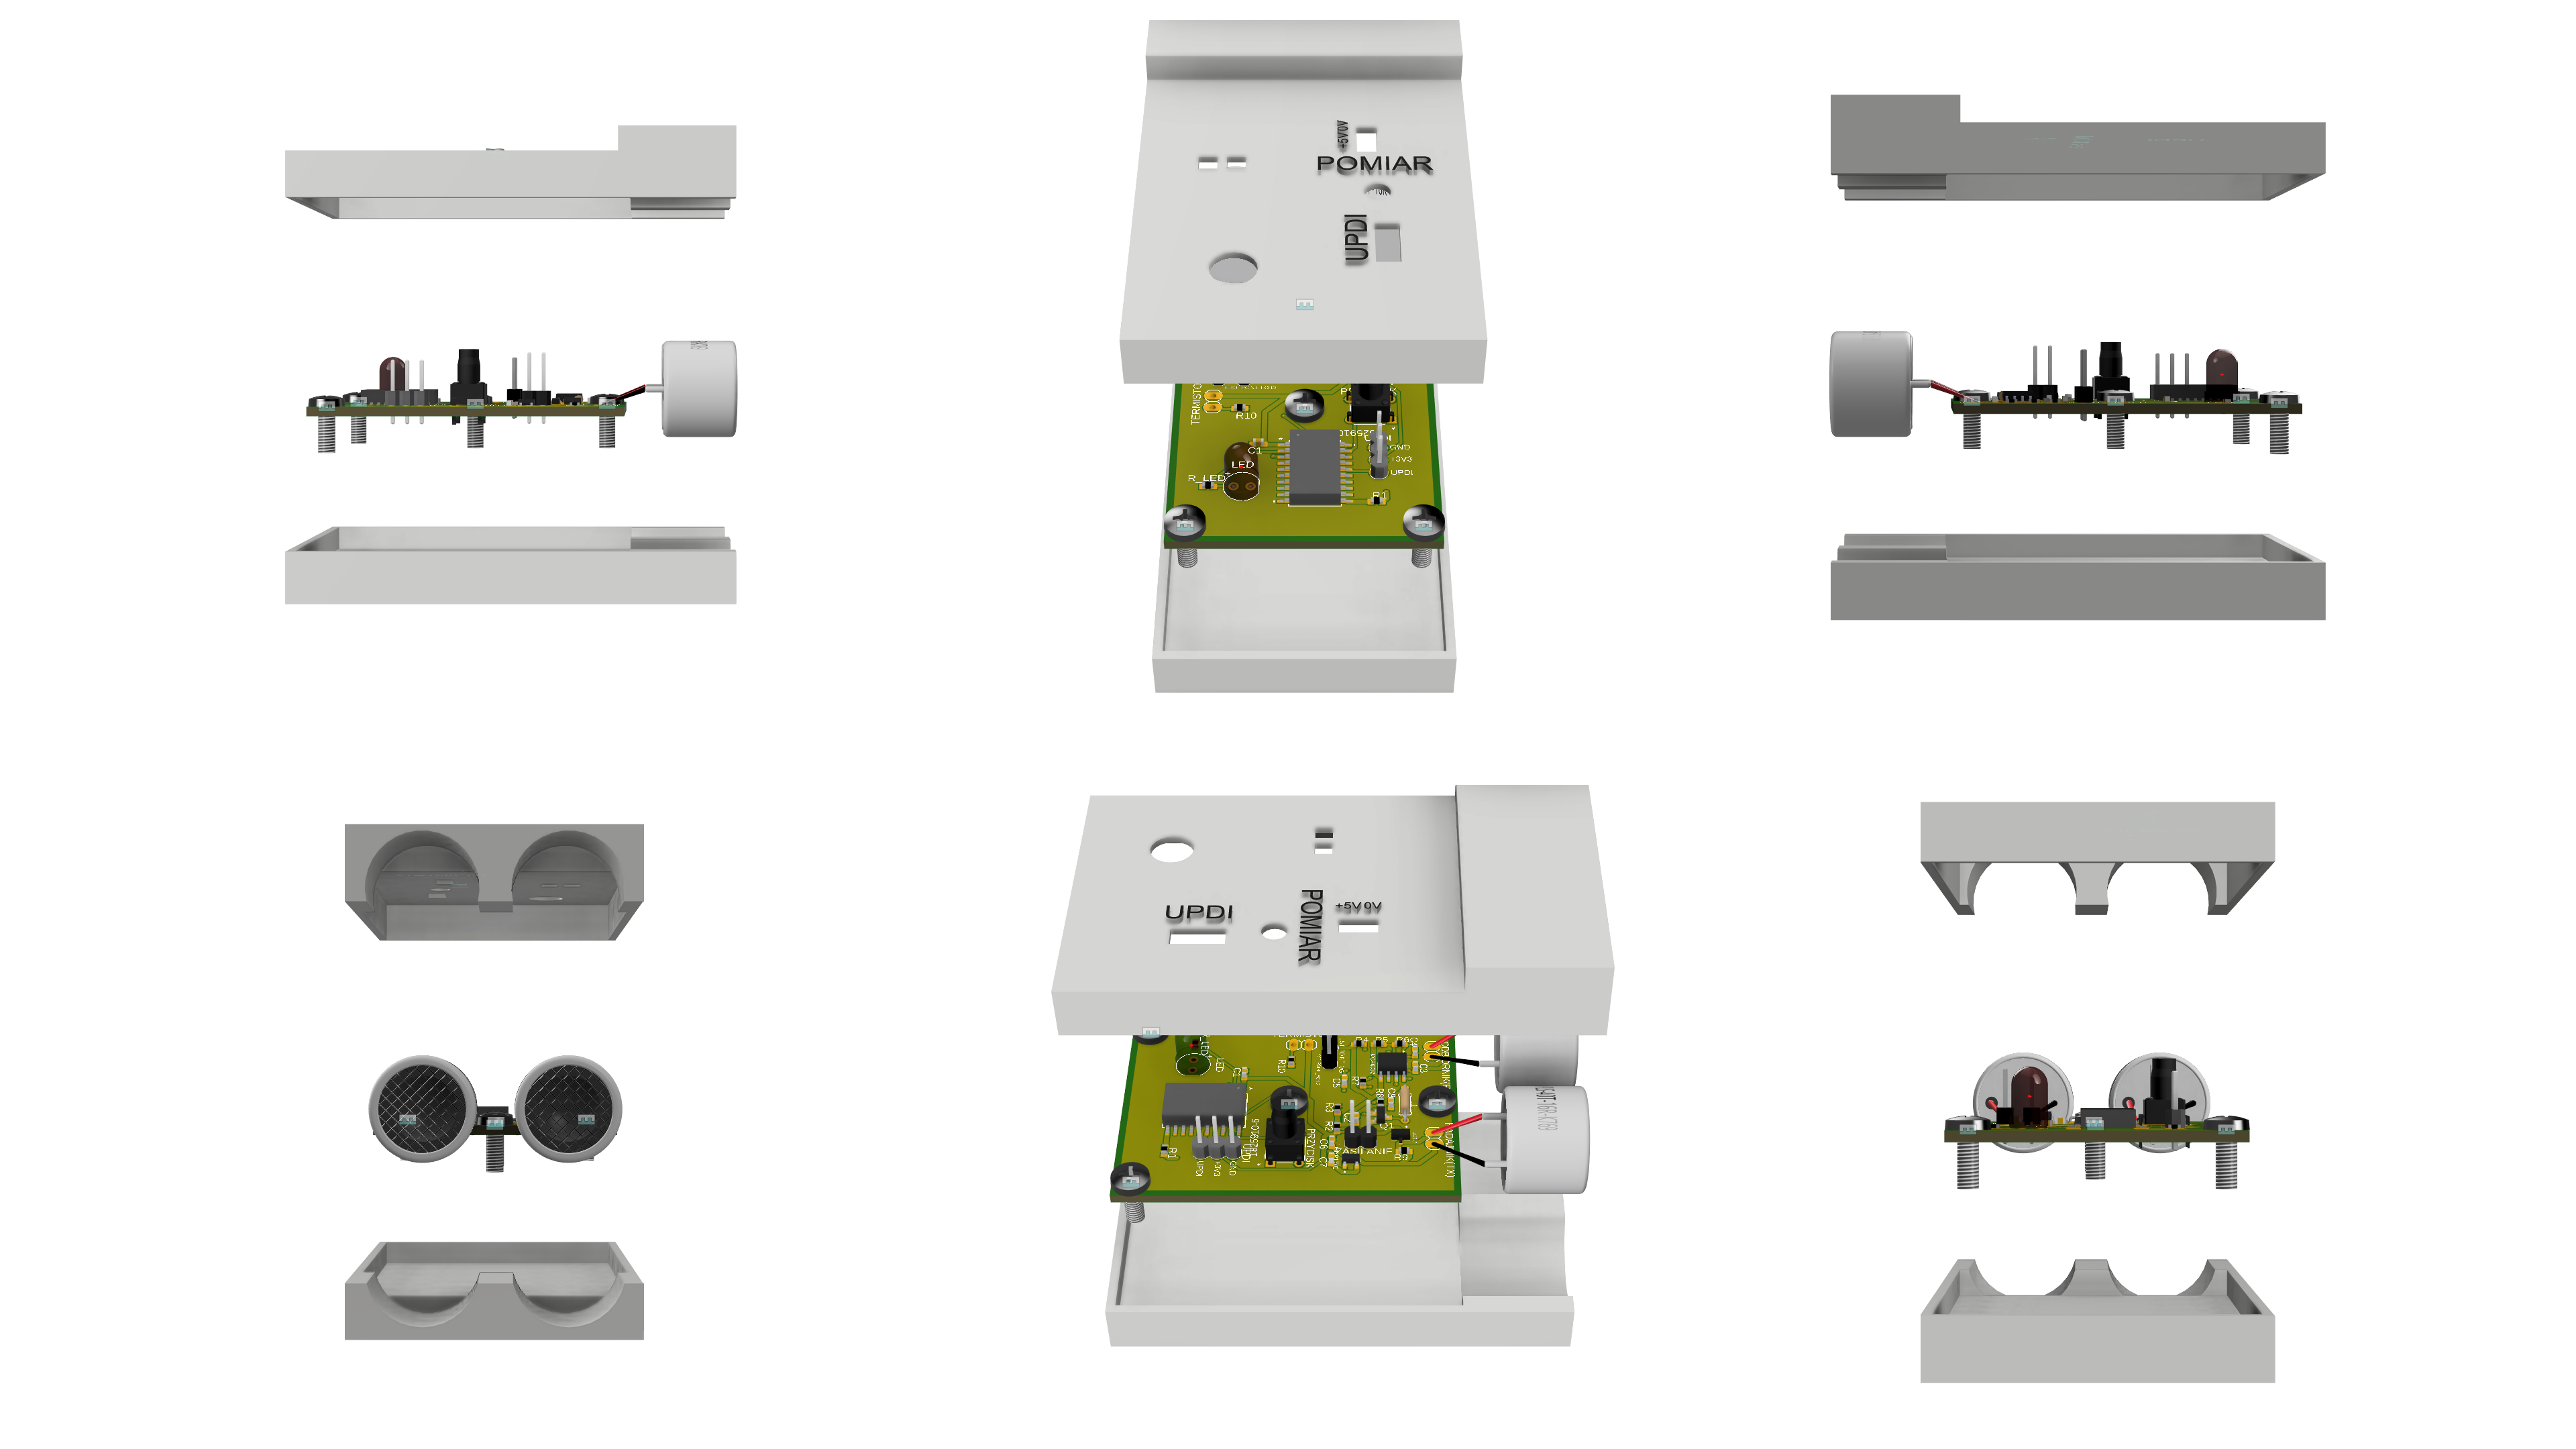
\includegraphics[width=0.75\textwidth]{obudowa_render_open.png}
		\caption{Render obudowy --- widok z~otwartą pokrywą.
			Widoczna płytka PCB zamontowana na czterech słupkach M3
			oraz ułożenie przetworników US w~otworach przedniej ścianki.}
		\label{fig:obudowa_open}
	\end{figure}
	
	\textit{Uwaga:} Wymiary obudowy oraz rozmiar otworów zostaną
	zweryfikowane po wykonaniu prototypu PCB w~Etapie~2. Pliki STL
	zostaną udostępnione wraz z~dokumentacją prototypu.
	
	
	% ══════════════════════════════════════════════════════════════
	% SEKCJA 5: ALGORYTM OPROGRAMOWANIA
	% ══════════════════════════════════════════════════════════════
	\clearpage
	\section{Algorytm oprogramowania}
	\label{sec:algorytm}
	
	\subsection{Architektura oprogramowania}
	
	Program mikrokontrolera został zaprojektowany w~języku C (AVR-GCC) z~podziałem
	na moduły:
	
	\begin{table}[H]
		\centering
		\caption{Moduły oprogramowania}
		\label{tab:moduly_sw}
		\begin{tabular}{lll}
			\toprule
			\textbf{Moduł} & \textbf{Plik} & \textbf{Funkcja} \\
			\midrule
			main & \texttt{main.c} & Pętla główna, inicjalizacja \\
			us\_driver & \texttt{us\_driver.c/h} & Generacja burstu, detekcja echa \\
			phase\_meas & \texttt{phase\_meas.c/h} & Algorytm Goertzela, obliczenie fazy \\
			temp\_comp & \texttt{temp\_comp.c/h} & Odczyt NTC, kompensacja $v(T)$ \\
			filter & \texttt{filter.c/h} & Filtr medianowy, uśrednianie \\
			uart & \texttt{uart.c/h} & Komunikacja USART \\
			power & \texttt{power.c/h} & Zarządzanie trybami uśpienia \\
			\bottomrule
		\end{tabular}
	\end{table}
	
	\subsection{Diagram przepływu}
	
	\noindent Poniższy diagram przedstawia pełny cykl pomiarowy --- od inicjalizacji,
	przez akwizycję i~przetwarzanie sygnału, po transmisję wyniku i~uśpienie mikrokontrolera.
	
	\begin{figure}[H]
		\centering
		\begin{tikzpicture}[
			node distance=0.6cm,
			startstop/.style={rectangle, rounded corners, draw, fill=NavyBlue!15,
				text width=4.5cm, align=center, minimum height=0.55cm, font=\footnotesize},
			process/.style={rectangle, draw, fill=white,
				text width=4.8cm, align=center, minimum height=0.55cm, font=\footnotesize},
			decision/.style={diamond, draw, fill=orange!15,
				text width=2.2cm, align=center, aspect=2.2, font=\footnotesize},
			io/.style={trapezium, draw, fill=Maroon!10, trapezium left angle=70,
				trapezium right angle=110, text width=3.5cm, align=center,
				minimum height=0.55cm, font=\footnotesize},
			arrow/.style={->, >=Stealth, semithick}
			]
			\node[startstop] (init) {Inicjalizacja CLK, TCA0,\\TCB0, ADC0, USART};
			\node[process, below=of init] (temp) {Odczyt NTC (ADC, 4$\times$ oversample)\\$T \to v(T)$};
			\node[process, below=of temp] (burst) {TCA0: Nadaj burst\\$N=8$ cykli @ 40\,kHz};
			\node[process, below=of burst] (tof) {TCB0: Czekaj na echo\\$t_{ToF} \to D_{coarse}$};
			\node[decision, below=0.8cm of tof] (echo_ok) {Echo\\wykryte?};
			\node[process, right=1.5cm of echo_ok, font=\footnotesize] (err) {Błąd: brak echa};
			\node[process, below=0.8cm of echo_ok] (adc_win) {Otwórz okno pomiarowe\\ADC: $K$ próbek echa};
			\node[process, below=of adc_win] (goertzel) {Algorytm Goertzela $\to \varphi$};
			\node[process, below=of goertzel] (fusion) {Fuzja: $D = n \cdot \lambda/2 + D_{fine}$};
			\node[decision, below=0.8cm of fusion] (med_ok) {Zebrano\\$M$ pomiarów?};
			\node[process, below=0.8cm of med_ok] (filter) {Filtr medianowy $\to D_{filtered}$};
			\node[io, below=of filter] (uart) {USART TX: ,,D=XXX.X mm''};
			\node[startstop, below=of uart] (sleep) {STANDBY SLEEP\\RTC wakeup $\to T_{cycle}$};
			
			\draw[arrow] (init) -- (temp);
			\draw[arrow] (temp) -- (burst);
			\draw[arrow] (burst) -- (tof);
			\draw[arrow] (tof) -- (echo_ok);
			\draw[arrow] (echo_ok) -- node[right, font=\scriptsize] {TAK} (adc_win);
			\draw[arrow] (echo_ok) -- node[above, font=\scriptsize] {NIE} (err);
			\draw[arrow] (err.south) |- (sleep.east);
			\draw[arrow] (adc_win) -- (goertzel);
			\draw[arrow] (goertzel) -- (fusion);
			\draw[arrow] (fusion) -- (med_ok);
			\draw[arrow] (med_ok) -- node[right, font=\scriptsize] {TAK ($M=7$)} (filter);
			\draw[arrow] (med_ok.west) -- ++(-2,0) |- node[left, pos=0.25, font=\scriptsize] {NIE} (temp.west);
			\draw[arrow] (filter) -- (uart);
			\draw[arrow] (uart) -- (sleep);
			\draw[arrow] (sleep.west) -- ++(-2.8,0) |- (temp.west);
		\end{tikzpicture}
		\caption{Diagram przepływu programu mikrokontrolera. Każdy wynik końcowy
			jest medianą z~$M = 7$ pomiarów jednostkowych. Alternatywnie pomiar może
			być wyzwalany przyciskiem na pinie PA7 (Pin Change interrupt ze Standby,
			patrz Tab.~\ref{tab:pinout}) --- tryb opcjonalny, nie zmienia architektury
			algorytmu.}
		\label{fig:flowchart}
	\end{figure}
	
	\subsection{Algorytm Goertzela --- wyznaczanie fazy sygnału echa}
	\label{sec:goertzel}
	
	Do wyznaczenia fazy sygnału echa przy częstotliwości $f_0 = \SI{40}{\kilo\hertz}$
	zastosowano \textbf{algorytm Goertzela} --- wydajną obliczeniowo wariant DFT
	dla pojedynczej częstotliwości. W~porównaniu z~pełnym FFT, algorytm Goertzela
	wymaga jedynie $O(N)$ operacji mnożenia i~dodawania oraz minimalnej ilości
	pamięci (${\sim}3$ zmienne stanu), co czyni go idealnym dla ATtiny1616.
	
	\subsubsection{Podstawy matematyczne}
	
	Algorytm oblicza składową Fouriera sygnału $x[n]$ przy znormalizowanej
	częstotliwości $k = N \cdot f_0 / f_s$, gdzie $N$ to liczba próbek,
	$f_s$ to częstotliwość próbkowania.
	
	Rekurencja Goertzela:
	\begin{equation}
		s[n] = x[n] + 2\cos\!\left(\frac{2\pi k}{N}\right) \cdot s[n-1] - s[n-2]
		\label{eq:goertzel_recur}
	\end{equation}
	
	z~warunkami początkowymi $s[-1] = s[-2] = 0$.
	
	Po przetworzeniu wszystkich $N$ próbek, składowa zespolona:
	\begin{equation}
		X[k] = s[N-1] - e^{-j2\pi k/N} \cdot s[N-2]
		\label{eq:goertzel_result}
	\end{equation}
	
	Faza sygnału:
	\begin{equation}
		\varphi = \arctan\!\left(\frac{\text{Im}(X[k])}{\text{Re}(X[k])}\right)
		= \text{atan2}\!\left(\text{Im}(X[k]),\, \text{Re}(X[k])\right)
		\label{eq:goertzel_phase}
	\end{equation}
	
	gdzie:
	\begin{align}
		\text{Re}(X[k]) &= s[N-1] - s[N-2] \cdot \cos(2\pi k / N) \label{eq:re} \\
		\text{Im}(X[k]) &= s[N-2] \cdot \sin(2\pi k / N) \label{eq:im}
	\end{align}
	
	\subsubsection{Parametry implementacji}
	
	\begin{table}[H]
		\centering
		\caption{Parametry algorytmu Goertzela w~projekcie}
		\label{tab:goertzel_params}
		\begin{tabularx}{\textwidth}{l r X}
			\toprule
			\textbf{Parametr} & \textbf{Wartość} & \textbf{Uzasadnienie} \\
			\midrule
			$f_s$ & ${\sim}\SI{96}{\kilo\hertz}$ & $f_{CLK\_ADC}/13 = 1{,}25\,\text{MHz}/13$ (w~spec.\ 10-bit) \\
			$N$ & 19 & ${\sim}2{,}4$ próbki/cykl $\times$ 8 cykli echa \\
			$k$ & ${\approx}\,7{,}92$ & $N \cdot f_0/f_s$; niecałkowite --- Goertzel akceptuje $k \in \mathbb{R}$ \\
			$\cos(2\pi k/N)$ & ${\approx}\,-0{,}998$ & Bliskie $-1$; mnożenie wymagane w~rekurencji \\
			Czas obliczeń & ${\sim}\SI{80}{\micro\second}$ & 16-bit stałoprzecinkowe (z~mnożeniem) \\
			Zużycie RAM & ${\sim}\SI{60}{\byte}$ & 3 zmienne int32 + bufor 19 próbek \\
			\bottomrule
		\end{tabularx}
	\end{table}
	
	\textbf{Uwaga implementacyjna:} Dla niecałkowitego $k \approx 7{,}92$ współczynnik
	$\cos(2\pi k/N) \approx -0{,}998$, co jest bliskie $-1$, ale \textbf{nie pozwala
		na eliminację mnożenia} z~pętli rekurencyjnej (w~odróżnieniu od idealnego
	przypadku $k = N/4$, gdzie $\cos = 0$). Rekurencja przyjmuje pełną postać:
	\begin{equation}
		s[n] = x[n] + 2\cos\!\left(\frac{2\pi k}{N}\right) \cdot s[n-1] - s[n-2]
		\label{eq:goertzel_full}
	\end{equation}
	
	Współczynnik $W = 2\cos(2\pi k/N)$ jest wyliczany jednorazowo przed pętlą
	i~przechowywany w~formacie stałoprzecinkowym Q1.14 (\SI{2}{\byte}).
	Mnożenie 16-bit $\times$ 16-bit realizowane jest przez sprzętowy mnożnik AVR
	(2-cyklowy \texttt{MUL}/\texttt{MULS}), co daje czas pętli ${\sim}\SI{4}{\micro\second}$/próbkę,
	łącznie ${\sim}\SI{80}{\micro\second}$ dla $N = 19$ próbek --- nadal pomijalny
	wobec czasu cyklu pomiarowego (\SI{5}{\milli\second}).
	
	\textit{Optymalizacja na Etap~2:} Jeśli eksperymentalna weryfikacja prototypu
	potwierdzi możliwość pracy ADC z~lekko podwyższonym $f_{CLK\_ADC} \approx
	\SI{1,56}{\mega\hertz}$ (DUTYCYC = 0, DS sekcja~30.5.17), wówczas
	osiągalny wariant $f_s = \SI{120}{\kilo\hertz}$ ($K = 3$ próbki/cykl)
	pozwoli użyć $N = 24$, $k = 8$, z~$\cos(2\pi \cdot 8/24) = \cos(2\pi/3) = -0{,}5$
	--- uproszczenie mnożenia do przesunięcia bitowego.
	
	\subsubsection{Pseudokod}
	
	\begin{lstlisting}[caption={Algorytm Goertzela --- pelna rekurencja dla $k \approx 7{,}92$, $N = 19$},
		label={lst:goertzel}]
		// Probkowanie ADC w oknie pomiarowym (ISR ADC)
		#define N_GOERTZEL 19
		int16_t samples[N_GOERTZEL];  // 19 probek @ ~96 kHz
		
		// Wspolczynnik Goertzela: W = 2*cos(2*pi*k/N), k = 19*40000/96154
		// W ~= 2 * (-0.998) = -1.996, w Q1.14: W_Q14 = -32702
		#define W_Q14 (-32702)  // 2*cos(2*pi*7.92/19) w Q1.14
		
		int32_t s0 = 0, s1 = 0, s2 = 0;
		for (uint8_t n = 0; n < N_GOERTZEL; n++) {
			s0 = (int32_t)samples[n]
			+ (((int32_t)W_Q14 * s1) >> 14)  // mnozenie Q1.14
			- s2;
			s2 = s1;
			s1 = s0;
		}
		
		// Skladowe Re i Im
		// cos_k = cos(2*pi*k/N), sin_k = sin(2*pi*k/N)
		// Prekalkulowane w Q14: cos_k_Q14, sin_k_Q14
		int32_t re = s1 - ((int32_t)cos_k_Q14 * s2 >> 14);
		int32_t im = (int32_t)sin_k_Q14 * s2 >> 14;
		
		// Faza (atan2 w arytmetyce staloprzecinkowej)
		int16_t phase_deg = atan2_fixed(im, re);  // wynik w 0.1 stopnia
		
		// Odleglosc fine
		int32_t d_fine_um = (int32_t)phase_deg * lambda_half_um / 3600;
	\end{lstlisting}
	
	\textbf{Implementacja \texttt{atan2\_fixed()}:} Funkcja arcus tangens
	w~arytmetyce stałoprzecinkowej. Planowane są dwa warianty do przetestowania
	w~Etapie~2:
	
	\begin{itemize}[nosep]
		\item \textbf{LUT:} tablica 256 wpisów $\times$ \SI{1}{\byte}
		= \SI{256}{\byte} Flash, z~interpolacją liniową między wpisami.
		Dokładność $< \SI{0,5}{\degree}$ ($\SI{8,7}{\milli\radian}$),
		co przy $\lambda/2 = \SI{4,29}{\milli\metre}$ odpowiada błędowi
		odległości $< \SI{0,006}{\milli\metre}$ --- pomijalny wobec
		pozostałych źródeł niepewności. Czas: ${\sim}\SI{10}{\micro\second}$.
		\item \textbf{CORDIC:} 16 iteracji, brak tablicy LUT, dokładność
		${\sim}0{,}005^{\circ}$. Czas: ${\sim}\SI{30}{\micro\second}$.
		Kosztem dłuższego obliczenia eliminuje zużycie Flash na tablicę.
	\end{itemize}
	
	Oba warianty mieszczą się w~budżecie Flash (\SI{16}{\kilo\byte}) i~nie wpływają
	istotnie na czas cyklu pomiarowego ($t_{active} = \SI{5}{\milli\second}$).
	
	\subsection{Filtracja wyników --- filtr medianowy}
	\label{sec:filtr}
	
	W~celu redukcji szumu pomiarowego i~eliminacji wartości odstających (outliers
	spowodowanych np.\ odbiciami wielokrotnymi) zastosowano filtr medianowy
	z~oknem $M = 7$ pomiarów.
	
	Filtr medianowy jest odporny na impulsowe zakłócenia (w~odróżnieniu od średniej
	arytmetycznej) i~nie wymaga znajomości rozkładu szumu. Algorytm sortowania
	dla $M = 7$ realizowany jest metodą sieci sortujących (sorting network) o~stałej
	liczbie porównań $C = 16$ i~zamian $S \leq 16$, co zajmuje ${\sim}\SI{15}{\micro\second}$.
	
	Po filtracji medianowej stosowana jest opcjonalna \textbf{wykładnicza średnia
		krocząca} (EMA) z~parametrem $\alpha = 0{,}3$:
	\begin{equation}
		D_{EMA}[k] = \alpha \cdot D_{median}[k] + (1-\alpha) \cdot D_{EMA}[k-1]
		\label{eq:ema}
	\end{equation}
	
	co wygładza wynik przy zachowaniu szybkiej reakcji na zmiany odległości.
	
	\subsection{Procedura kalibracji}
	\label{sec:kalibracja}
	
	Przed pierwszym użyciem urządzenie wykonuje jednorazową procedurę kalibracyjną
	mającą na celu kompensację systematycznych błędów:
	
	\begin{enumerate}[nosep]
		\item \textbf{Kalibracja offsetu ToF} --- pomiar przy znanej odległości
		referencyjnej (np.\ \SI{20}{\centi\metre}), wyznaczenie offsetu
		$t_{offset}$ wynikającego z~opóźnień elektroniki i~ring-downu nadajnika.
		\item \textbf{Kalibracja fazy} --- pomiar przy dwóch znanych odległościach
		różniących się o~$\lambda/2$, weryfikacja liniowości pomiaru fazowego.
		\item \textbf{Współczynnik korekcji wzmocnienia} --- opcjonalne dopasowanie
		krzywej $D_{measured} = a \cdot D_{raw} + b$ metodą najmniejszych
		kwadratów dla 3--5 punktów referencyjnych.
	\end{enumerate}
	
	Parametry kalibracyjne zapisywane są w~pamięci EEPROM ATtiny1616
	(\SI{256}{\byte} dostępne). Szacowane zużycie pamięci EEPROM:
	
	\begin{table}[H]
		\centering
		\caption{Szacowane wykorzystanie EEPROM na dane kalibracyjne}
		\label{tab:eeprom_usage}
		\begin{tabular}{lrl}
			\toprule
			\textbf{Parametr} & \textbf{Rozmiar} & \textbf{Typ danych} \\
			\midrule
			Offset ToF ($t_{offset}$) & 4\,B & \texttt{int32\_t} ($\si{\micro\second}$) \\
			Współczynniki korekcji $a$, $b$ & 8\,B & 2 $\times$ \texttt{int32\_t} (Q16.16) \\
			Temperatura referencyjna $T_0$ & 2\,B & \texttt{int16\_t} ($0{,}1\,^\circ$C) \\
			LUT wielopunktowa (10~pkt) & 40\,B & 10 $\times$ 4\,B \\
			CRC16 kontrolna & 2\,B & \texttt{uint16\_t} \\
			\midrule
			\textbf{Łącznie} & \textbf{56\,B} & z~256\,B dostępnych (\SI{22}{\percent}) \\
			\bottomrule
		\end{tabular}
	\end{table}
	
	\subsubsection{Szacunek zużycia pamięci Flash i~SRAM}
	\label{sec:flash_sram}
	
	Mikrokontroler ATtiny1616 dysponuje \SI{16}{\kilo\byte} Flash i~\SI{2}{\kilo\byte}
	SRAM. Poniższa tabela przedstawia szacunkowe zapotrzebowanie poszczególnych
	modułów firmware na pamięć programu i~danych.
	
	\begin{table}[H]
		\centering
		\caption{Szacunkowe zużycie pamięci Flash i~SRAM}
		\label{tab:flash_sram}
		\begin{tabular}{l r r l}
			\toprule
			\textbf{Moduł} & \textbf{Flash [B]} & \textbf{SRAM [B]} & \textbf{Uwagi} \\
			\midrule
			Inicjalizacja peryferiów    & ${\sim}400$  & 0        & CLKCTRL, TCA, TCB, ADC, AC, EVSYS \\
			Algorytm Goertzela          & ${\sim}600$  & 32       & 4 zmienne Q16.16 (akumulatory) \\
			Tabela LUT \texttt{atan2}   & 256          & 0        & 256\,B w~Flash (stałe) \\
			Obliczenia fazowe i~fuzja   & ${\sim}500$  & 24       & $D_{ToF}$, $D_{fine}$, $n$, reszta $r$ \\
			Filtr medianowy ($M = 7$)   & ${\sim}200$  & 28       & bufor 7 $\times$ \texttt{int32\_t} \\
			Kompensacja NTC             & ${\sim}300$  & 8        & model B-parametrowy, interpolacja \\
			Obsługa USART (TX)          & ${\sim}250$  & 32       & bufor ramki ASCII \\
			Obsługa EEPROM (kalibracja) & ${\sim}200$  & 0        & zapis/odczyt parametrów \\
			Sterownik LED + przycisk    & ${\sim}100$  & 2        & GPIO, debouncing \\
			Zarządzanie energią (sleep) & ${\sim}150$  & 0        & Standby, budzenie RTC \\
			Stos + zmienne globalne     & ---          & ${\sim}128$ & stos wywołań ISR \\
			\midrule
			\textbf{Łącznie (szacunek)} & \textbf{${\sim}$2\,960} & \textbf{${\sim}$254} &  \\
			\midrule
			\textbf{Dostępne}           & 16\,384      & 2\,048   &  \\
			\textbf{Wykorzystanie}      & ${\sim}\SI{18}{\percent}$ & ${\sim}\SI{12}{\percent}$ & znaczny zapas \\
			\bottomrule
		\end{tabular}
	\end{table}
	
	Wykorzystanie pamięci na poziomie ${\sim}\SI{18}{\percent}$ Flash
	i~${\sim}\SI{12}{\percent}$ SRAM pozostawia znaczny zapas na ewentualne
	rozszerzenia firmware (np.\ wielopunktowa kalibracja LUT, filtr Kalmana,
	dodatkowe tryby pracy).
	
	\subsubsection{Kluczowe rejestry konfiguracyjne mikrokontrolera}
	\label{sec:rejestry}
	
	Poniższa tabela przedstawia wartości inicjalizacyjne najważniejszych
	rejestrów peryferyjnych ATtiny1616, zapisywane w~procedurze \texttt{init\_hw()}
	po resecie. Zestawienie demonstruje konfigurację na poziomie rejestrowym.
	
	\begin{table}[H]
		\centering
		\caption{Kluczowe rejestry konfiguracyjne ATtiny1616}
		\label{tab:rejestry}
		\footnotesize
		\begin{tabularx}{\textwidth}{l l l X}
			\toprule
			\textbf{Peryferium} & \textbf{Rejestr} & \textbf{Wartość} & \textbf{Znaczenie} \\
			\midrule
			CLKCTRL & MCLKCTRLA   & \texttt{0x00}  & OSC20M jako źródło zegara \\
			& MCLKCTRLB   & \texttt{0x01}  & Prescaler $\div 2$ $\to$ $f_{CLK} = \SI{10}{\mega\hertz}$ \\
			\midrule
			TCA0    & CTRLA       & \texttt{0x01}  & Enable, prescaler $\div 1$ \\
			& CTRLB       & \texttt{0x13}  & Single-slope PWM, CMP0 enabled (WO0) \\
			& PER         & \texttt{249}   & Okres $= 250$ taktów $\to f_{PWM} = \SI{40}{\kilo\hertz}$ \\
			& CMP0        & \texttt{124}   & Wypełnienie 50\% (sygnał nadajnika) \\
			\midrule
			TCB0    & CTRLA       & \texttt{0x01}  & Enable, CLK\_PER \\
			& CTRLB       & \texttt{0x03}  & Input Capture Frequency Measurement \\
			& EVCTRL      & \texttt{0x01}  & Capture on event (AC0 output) \\
			\midrule
			ADC0    & CTRLA       & \texttt{0x01}  & Enable, 10-bit \\
			& CTRLB       & \texttt{0x00}  & Brak akumulacji \\
			& CTRLC       & \texttt{0x43}  & $V_{ref}$ = VDD, prescaler $\div 64$ $\to f_{ADC} = \SI{156}{\kilo\hertz}$ \\
			& MUXPOS      & \texttt{0x00--0x07} & AIN0 (echo) / AIN7 (NTC) \\
			\midrule
			AC0     & CTRLA       & \texttt{0x41}  & Enable, HYSMODE = 25\,mV \\
			& MUXCTRLA    & \texttt{0x01}  & AINP0 (wyjście toru RX), AINN = DACREF \\
			& DACREF      & \texttt{var.}  & Próg detekcji $\approx 15\%\,V_{DD}$ powyżej $V_{DD}/2$ \\
			\midrule
			EVSYS   & CHANNEL0    & \texttt{0x1C}  & Generator: AC0 OUT \\
			& USEREVOUTA  & \texttt{0x01}  & User: TCB0 CAPT (pomiar ToF) \\
			\midrule
			SLPCTRL & CTRLA       & \texttt{0x05}  & Sleep mode = Standby, Sleep Enable \\
			\midrule
			RTC     & CTRLA       & \texttt{0x01}  & Enable, prescaler $\div 1$ \\
			& PER         & \texttt{var.}  & Okres budzenia (domyślnie \SI{50}{\milli\second}) \\
			& INTCTRL     & \texttt{0x01}  & Overflow interrupt (budzenie z~sleep) \\
			\bottomrule
		\end{tabularx}
	\end{table}
	
	\subsection{Komunikacja USART}
	\label{sec:usart}
	
	Wynik pomiaru transmitowany jest przez USART0 (pin PA1/TXD) w~formacie ASCII:
	
	\begin{lstlisting}[caption={Format ramki wyjściowej USART}, label={lst:uart_frame}]
		// Format: "D=XXX.X mm\r\n"
		// Przyklad: "D=234.7 mm\r\n"
		// Baudrate: 9600 bps (8N1)
		// Odczyt: dowolny terminal szeregowy (PuTTY, screen, minicom)
		// Podlaczenie: UPDI header pin 1 (TX) + GND
	\end{lstlisting}
	
	Transmisja jednej ramki (${\sim}16$ znaków @ 9600\,bps) trwa ${\sim}\SI{17}{\milli\second}$.
	W~trybie oszczędnym USART jest wyłączany między transmisjami.
	
	
	% ══════════════════════════════════════════════════════════════
	% SEKCJA 6: BUDŻET KOSZTÓW
	% ══════════════════════════════════════════════════════════════
	\section{Budżet kosztów}
	\label{sec:koszty}
	
	\begin{table}[H]
		\centering
		\caption{Koszt elementów urządzenia (wg regulaminu i~cen brutto sklepów)}
		\label{tab:koszty}
		\begin{tabularx}{\textwidth}{l l r r r X}
			\toprule
			\textbf{Element} & \textbf{Ozn.} & \textbf{Ilość} &
			\textbf{Cena/szt.} & \textbf{Suma} & \textbf{Źródło} \\
			\midrule
			\multicolumn{6}{l}{\textit{R, L, C, tranzystory, diody --- \SI{0,15}{PLN}/szt.\ (regulamin):}} \\
			\midrule
			Rezystory 0603 & R1--R10 & 11 & 0,15 & 1,65 & regulamin \\
			Kondensatory 0603 & C1--C8 & 8 & 0,15 & 1,20 & regulamin \\
			Cewka \SI{10}{\micro\henry} & L1 & 1 & 0,15 & 0,15 & regulamin \\
			BC817-40 (NPN) & BC817 & 1 & 0,15 & 0,15 & regulamin \\
			BSS84 (P-MOSFET) & Q2 & 1 & 0,15 & 0,15 & regulamin \\
			Rezystor R8 (pullup gate Q2) & R8 & 1 & 0,15 & 0,15 & regulamin \\
			LED czerwona & LED & 1 & 0,15 & 0,15 & regulamin \\
			\midrule
			\multicolumn{6}{l}{\textit{Wzmacniacze operacyjne --- \SI{1,00}{PLN}/szt.\ (regulamin):}} \\
			\midrule
			MCP6002-I/SN & MCP6002 & 1 & 1,00 & 1,00 & regulamin \\
			\midrule
			\multicolumn{6}{l}{\textit{PCB --- cena regulaminowa:}} \\
			\midrule
			Płytka drukowana & PCB & 1 & 15,00 & 15,00 & regulamin \\
			\midrule
			\multicolumn{6}{l}{\textit{Pozostałe --- ceny brutto, sklepy UE:}} \\
			\midrule
			ATtiny1616-SN & U1 & 1 & 5,90 & 5,90 &
			\href{https://www.tme.eu/pl/details/attiny1616-sn/rodzina-avr-8-bit/microchip-technology/}{TME} \\
			MCP1700T-3302E/TT & U2 & 1 & 3,70 & 3,70 &
			\href{https://www.tme.eu/pl/details/mcp1700t-3302e_tt/stabilizatory-ldo-nienastawne/microchip-technology/}{TME} \\
			Przycisk 1825910-6 & SW1 & 1 & 0,50 & 0,50 &
			\href{https://www.tme.eu/pl/details/1825910-6/przelaczniki-tact/te-connectivity/}{TME} \\
			Listwa goldpin 1$\times$40 & JP & 1 & 1,31 & 1,31 &
			\href{https://www.tme.eu/pl/details/zl201-40g/listwy-i-gniazda-kolkowe/connfly/ds1021-1-40sf11-b/}{TME} \\
			Przetworniki US 40\,kHz (para) & TX+RX & 1 & 11,50 & 11,50 &
			\href{https://botland.com.pl/ultradzwiekowe-czujniki-odleglosci/1209-czujniki-ultradzwiekowe-16mm-komplet-5904422355920.html}{Botland} \\
			NTC 10\,k$\Omega$ (NTCM-HP-10K) & NTC & 1 & 1,22 & 1,22 &
			\href{https://www.tme.eu/pl/details/ntcm-hp-10k-1\%25/termistory-ntc-pomiarowe-tht/sr-passives/}{TME} \\
			\midrule
			\multicolumn{4}{r}{\textbf{RAZEM:}} & \textbf{43,73} & PLN \\
			\bottomrule
		\end{tabularx}
	\end{table}
	
	Punkty za cenę elementów:
	\begin{equation}
		P_{cena} = \min\!\left(50,\; \frac{50 \times 50}{43{,}73}\right)
		= \min(50;\; 57{,}2) = \textbf{50~pkt~(max)}
		\label{eq:pkt_cena}
	\end{equation}
	
	
	% ══════════════════════════════════════════════════════════════
	% SEKCJA 7: BUDŻET MOCY
	% ══════════════════════════════════════════════════════════════
	\section{Budżet mocy}
	\label{sec:moc}
	
	\subsection{Prąd pobierany przez poszczególne elementy}
	
	\begin{table}[H]
		\centering
		\caption{Szczegółowy budżet prądowy (dane z~kart katalogowych)}
		\label{tab:moc_detail}
		\begin{tabularx}{\textwidth}{l r r r X}
			\toprule
			\textbf{Element} & \textbf{$I_{active}$} & \textbf{$I_{sleep}$}
			& \textbf{$t_{active}$} & \textbf{Źródło danych} \\
			\midrule
			ATtiny1616 @ 10\,MHz, 3{,}3V
			& ${\sim}\SI{3,4}{\milli\ampere}$
			& \SI{0,7}{\micro\ampere}
			& \SI{5}{\milli\second}
			& DS Tab.~36-4 (3{,}1\,mA @ 3{,}0V; ${\sim}$3{,}4\,mA @ 3{,}3V) \\
			ATtiny1616 (Standby + RTC)
			&
			& \SI{0,7}{\micro\ampere}
			&
			& DS Tab.~36-5 (OSCULP32K, typ.) \\
			MCP6002 (oba kanały)
			& \SI{100}{\micro\ampere}
			& \SI{100}{\micro\ampere}
			& ciągły
			& DS, Tab.~1.1 \\
			MCP1700 ($I_q$)
			& \SI{1,6}{\micro\ampere}
			& \SI{1,6}{\micro\ampere}
			& ciągły
			& DS, Tab.~1 \\
			Nadajnik US (burst)
			& \SI{20}{\milli\ampere}
			& \SI{0}{\micro\ampere}
			& \SI{0,2}{\milli\second}
			& estymacja; \textbf{z~5V} (nie LDO) \\
			LED (puls)
			& \SI{3,3}{\milli\ampere}
			& \SI{0}{\micro\ampere}
			& \SI{1}{\milli\second}
			& $R_{LED} = \SI{1}{\kilo\ohm}$ \\
			\bottomrule
		\end{tabularx}
	\end{table}
	
	\subsection{Scenariusze pracy}
	
	\subsubsection{Scenariusz 1: Ciągły pomiar (bez uśpienia)}
	
	Przy ciągłym działaniu wszystkich elementów (@ \SI{3,3}{\volt}):
	\begin{equation}
		I_{avg,1} = I_{MCU} + I_{opamp} + I_{LDO} + I_{LED} \cdot D_{LED}
		= 3{,}4 + 0{,}1 + 0{,}002 + 3{,}3 \cdot 0{,}2 \approx \SI{4,2}{\milli\ampere}
	\end{equation}
	
	gdzie $D_{LED} = 0{,}2$ to szacowany współczynnik wypełnienia sygnalizacji LED
	(włączona na \SI{1}{\milli\second} co \SI{5}{\milli\second} cyklu pomiarowego).
	
	\textbf{Uwaga:} Nadajnik US jest zasilany bezpośrednio z~\SI{5}{\volt}
	(kolektor BC817 podłączony do +5V, nie przez LDO). Prąd nadajnika
	(20\,mA burst, duty cycle ${\sim}4\%$) nie obciąża stabilizatora MCP1700.
	Średni prąd nadajnika z~5V: $20 \cdot 0{,}04 = \SI{0,8}{\milli\ampere}$.
	
	\begin{align}
		P_{in,1} &= \frac{I_{avg,1} \cdot V_{3,3}}{\eta_{LDO}} + I_{TX,avg} \cdot V_{5V}
		= \frac{4{,}2 \cdot 3{,}3}{0{,}66} + 0{,}8 \cdot 5 = 21{,}0 + 4{,}0 = \SI{25,0}{\milli\watt} \notag \\
		P_{pkt,1} &= 100/25{,}0 \approx \textbf{4,0~pkt} \notag
	\end{align}
	
	\subsubsection{Scenariusz 2: Pomiar okresowy ze sleep mode (planowany)}
	
	Cykl pomiarowy: $T_{cycle} = \SI{100}{\milli\second}$, czas aktywny
	$t_{active} = \SI{5}{\milli\second}$ (burst + ToF + ADC + Goertzel + UART),
	czas uśpienia $t_{sleep} = \SI{95}{\milli\second}$ (tryb Standby z~RTC wakeup).
	
	Średni prąd mikrokontrolera (Standby z~RTC, $I_{standby} = \SI{0,7}{\micro\ampere}$):
	\begin{equation}
		I_{MCU,avg} = \frac{t_{active} \cdot I_{active} + t_{sleep} \cdot I_{sleep}}{T_{cycle}}
		= \frac{5 \cdot 3400 + 95 \cdot 0{,}7}{100} \approx \SI{171}{\micro\ampere}
		\label{eq:imcu_avg}
	\end{equation}
	
	Średni prąd całkowity (@ \SI{3,3}{\volt}, bez nadajnika):
	\begin{equation}
		I_{avg,2} = 171 + 100 + 1{,}6 + 3300 \cdot \frac{1}{100}
		\approx \SI{306}{\micro\ampere}
	\end{equation}
	
	Prąd nadajnika z~5V (średni): $I_{TX,avg} = 20000 \cdot 0{,}2 / 100 = \SI{40}{\micro\ampere}$.
	
	Moc pobierana z~zasilania \SI{5}{\volt}:
	\begin{align}
		P_{in,2} &= \frac{I_{avg,2} \cdot V_{3,3}}{\eta_{LDO}} + I_{TX,avg} \cdot V_{5V}
		= \frac{0{,}306 \cdot 3{,}3}{0{,}66} + 0{,}040 \cdot 5
		\approx 1{,}53 + 0{,}20 = \SI{1,7}{\milli\watt} \label{eq:moc_scen2} \\
		P_{pkt,2} &= \min(50,\; 100/1{,}7) \approx \textbf{50~pkt~(max)} \notag
	\end{align}
	
	\subsubsection{Scenariusz 3: Agresywna optymalizacja (cel)}
	
	Dodatkowe optymalizacje planowane w~Etapie~2:
	\begin{itemize}[nosep]
		\item Wyłączanie MCP6002 przez odcięcie zasilania pinem GPIO + P-MOSFET
		($I_{sleep,opamp} = \SI{0}{\micro\ampere}$)
		\item Redukcja $T_{cycle}$ do \SI{200}{\milli\second} (pomiar co 5/s)
		\item Taktowanie MCU na \SI{5}{\mega\hertz} w~fazie obliczeń
		(prescaler $\div 4$, $I_{active} \approx \SI{1,8}{\milli\ampere}$ @ 3{,}0V, DS Tab.~36-4; ${\sim}\SI{2,0}{\milli\ampere}$ @ 3{,}3V)
		\item Wyłączanie LED (wynik tylko przez UART)
	\end{itemize}
	
	Szacowany średni prąd:
	\begin{equation}
		I_{avg,3} \approx \SI{120}{\micro\ampere}, \quad
		P_{in,3} \approx \SI{0,8}{\milli\watt}, \quad
		P_{pkt,3} = \min(50, 100/0{,}8) \approx \textbf{50~pkt~(max)}
		\label{eq:moc_scen3}
	\end{equation}
	
	\textit{Uwaga:} Wyłączanie MCP6002 przez P-MOSFET (np.\ BSS84, \SI{0,15}{PLN} wg regulaminu
	--- ujęty w~BOM, Tab.~\ref{tab:koszty}) wymaga wydłużenia
	$t_{active}$ o~${\sim}\SI{2}{\milli\second}$ na czas stabilizacji wzmacniacza
	po włączeniu zasilania. Realistycznie $I_{avg,3} \approx \SIrange{120}{180}{\micro\ampere}$.
	
	
	% ══════════════════════════════════════════════════════════════
	% SEKCJA 8: ANALIZA BŁĘDÓW
	% ══════════════════════════════════════════════════════════════
	\section{Analiza błędów i~niepewność pomiaru}
	\label{sec:bledy}
	
	\subsection{Budżet niepewności}
	
	\begin{table}[H]
		\centering
		\caption{Szczegółowy budżet niepewności pomiaru @ $D = \SI{30}{\centi\metre}$, $T = \SI{20}{\celsius}$}
		\label{tab:bledy}
		\begin{tabularx}{\textwidth}{>{\raggedright\arraybackslash}p{3.8cm}rrX}
			\toprule
			\textbf{Źródło} & \textbf{$\sigma$ [\si{\milli\metre}]} & \textbf{Typ}
			& \textbf{Kompensacja / redukcja} \\
			\midrule
			Szum ADC (10-bit, 1\,LSB)
			& 0,10
			& Losowy
			& Oversampling $4\times$ ($\to \sigma/2$), Goertzel filtruje szum poza $f_0$ \\
			Niepewność pomiaru fazy
			& 0,15
			& Losowy
			& Uśrednianie z~$M=7$ pomiarów ($\to \sigma/\sqrt{7}$) \\
			Kompensacja temp.\ (resztkowa)
			& 0,05
			& Systematyczny
			& Termistor NTC z~oversamplingiem ($\Delta T < \SI{0,1}{\kelvin}$) \\
			Jitter zegara wewn.\ osc.
			& 0,12
			& Losowy
			& Kalibracja oscylatora, pomiar różnicowy ($\pm\SI{2}{\percent}$ @ 3V/25$^\circ$C, do $\pm\SI{5}{\percent}$ w~pełnym zakresie temp.) \\
			Kąt padania wiązki US
			& 0,20
			& Systematyczny
			& Mechaniczne ustawienie, karton $20\times20$\,cm redukuje wrażliwość \\
			Odbicia wielokrotne (multipath)
			& 0,30
			& Losowy
			& Filtr medianowy eliminuje outliers, bramkowanie czasowe \\
			Ring-down nadajnika (bliskie pole)
			& 0,15
			& Systematyczny
			& Kalibracja offsetu ToF, $D_{min} = \SI{10}{\centi\metre}$ (\SI{0,6}{\milli\second} --- wystarczający czas wygaszenia) \\
			Rozrzut $f_0$ przetworników
			& 0,10
			& Systematyczny
			& Jednorazowa kalibracja, zapis w~EEPROM \\
			\bottomrule
		\end{tabularx}
	\end{table}
	
	\subsection{Szacowany RMSE}
	
	Zakładając nieskorelowanie poszczególnych źródeł błędu, sumaryczna
	niepewność standardowa (przed filtracją):
	\begin{equation}
		\sigma_{total} = \sqrt{\sum_i \sigma_i^2}
		= \sqrt{0{,}10^2 + 0{,}15^2 + 0{,}05^2 + 0{,}12^2 + 0{,}20^2 + 0{,}30^2 + 0{,}15^2 + 0{,}10^2}
		\approx \SI{0,48}{\milli\metre}
		\label{eq:sigma_total}
	\end{equation}
	
	Po filtracji medianowej ($M = 7$) i~EMA ($\alpha = 0{,}3$), efektywna
	redukcja szumu losowego o~czynnik ${\sim}2{,}5$:
	\begin{equation}
		\boxed{RMSE_{est} \approx \SI{0,3}{\milli\metre} \text{ -- } \SI{0,8}{\milli\metre}}
		\label{eq:rmse_final}
	\end{equation}
	
	Dolna granica (0,3\,mm) odpowiada idealnemu scenariuszowi z~dobrze
	skalibrowanym urządzeniem; górna (0,8\,mm) --- warunkom niekontrolowanym
	z~odbiciami. W~obu przypadkach wynik jest znacząco lepszy niż osiągalny
	metodą prostego ToF (${\sim}\SI{3}{\milli\metre}$).
	
	\subsection{Analiza worst-case: odległość minimalna $D_{min} = \SI{10}{\centi\metre}$}
	\label{sec:worst_case_dmin}
	
	Odległość minimalna stanowi najtrudniejszy scenariusz pomiarowy, ponieważ
	echo powraca najszybciej --- kluczowe jest, czy ring-down nadajnika
	i~przejściówka toru RX zdążą wygasnąć przed nadejściem echa.
	
	\textbf{Budżet czasowy:}
	Czas przelotu dla $D_{min} = \SI{10}{\centi\metre}$ (w obie strony
	$2D = \SI{20}{\centi\metre}$) przy $v = \SI{343}{\metre\per\second}$:
	\begin{equation}
		t_{ToF,min} = \frac{2 \cdot D_{min}}{v} = \frac{2 \cdot 0{,}10}{343} = \SI{0,583}{\milli\second}
		\label{eq:tof_min}
	\end{equation}
	
	\textbf{Czas trwania burstu TX:}
	Nadajnik generuje 8 cykli @ \SI{40}{\kilo\hertz}, co trwa:
	\begin{equation}
		t_{burst} = \frac{8}{f_0} = \frac{8}{40\,000} = \SI{0,200}{\milli\second}
		\label{eq:t_burst}
	\end{equation}
	
	\textbf{Ring-down nadajnika:}
	Typowy czas ring-downu przetwornika piezoelektrycznego TCT-40 wynosi
	$\tau_{ring} \approx \SIrange{0,3}{0,5}{\milli\second}$ (tłumienie
	sygnału o~\SI{40}{\deci\bel}). W~najgorszym przypadku:
	\begin{equation}
		t_{ring,max} \approx \SI{0,5}{\milli\second}
		\label{eq:t_ring}
	\end{equation}
	
	\textbf{Margines czasowy:}
	Czas od zakończenia burstu do nadejścia echa:
	\begin{equation}
		\Delta t = t_{ToF,min} - t_{burst} = 0{,}583 - 0{,}200 = \SI{0,383}{\milli\second}
		\label{eq:dt_margin}
	\end{equation}
	
	Porównanie z~ring-downem: $\Delta t = \SI{0,383}{\milli\second}$
	vs.\ $t_{ring,max} = \SI{0,5}{\milli\second}$ --- ring-down nadajnika
	\textbf{nie zdąży w~pełni wygasnąć} przed nadejściem echa. Jednak
	zastosowane środki łagodzące zapewniają poprawny pomiar:
	
	\begin{enumerate}
		\item \textbf{Separacja przetworników:} Nadajnik (TX) i~odbiornik (RX)
		to osobne przetworniki, fizycznie odseparowane na PCB --- ring-down
		mechaniczny nie przechodzi bezpośrednio do toru RX.
		\item \textbf{Komparator AC0 z~progiem:} Próg detekcji ustawiony powyżej
		poziomu resztkowego ring-downu zapobiega fałszywemu wyzwoleniu.
		Ring-down na odbiorniku jest tłumiony o~${\sim}\SI{20}{\deci\bel}$
		dzięki separacji przetworników.
		\item \textbf{Okno pomiarowe firmware:} Pomiar ToF (TCB0) jest aktywowany
		dopiero po upływie $t_{blank} = \SI{0,4}{\milli\second}$ od początku
		burstu (blanking window), co eliminuje fałszywe wyzwolenia od
		ring-downu.
		\item \textbf{Offset kalibracyjny $t_{offset}$:} Kalibracja przy znanej
		odległości kompensuje systematyczne opóźnienia wynikające z~elektroniki
		i~ring-downu.
	\end{enumerate}
	
	W~efekcie pomiar przy $D_{min} = \SI{10}{\centi\metre}$ jest realizowalny,
	choć stanowi granicę możliwości układu --- RMSE przy tej odległości będzie
	wyższy niż w~środku zakresu pomiarowego ze względu na częściowe nakładanie
	się ring-downu z~początkiem echa.
	
	\subsubsection{Adaptacyjna długość burstu}
	\label{sec:adaptive_burst}
	
	Dodatkową optymalizacją planowaną w~firmware jest \textbf{adaptacyjna
		długość burstu TX} w~zależności od zmierzonej odległości. Algorytm działa
	w~dwóch krokach:
	
	\begin{enumerate}[nosep]
		\item \textbf{Pomiar wstępny} z~domyślnym burstem $N = 8$ cykli ---
		wyznaczenie przybliżonej odległości $D_{coarse}$ z~ToF.
		\item \textbf{Pomiar właściwy} z~adaptowaną długością burstu:
		\begin{itemize}[nosep]
			\item $D < \SI{15}{\centi\metre}$: $N = 4$ cykle
			($t_{burst} = \SI{0,100}{\milli\second}$, zysk
			$\SI{0,1}{\milli\second}$ marginesu)
			\item $\SI{15}{\centi\metre} \leq D < \SI{25}{\centi\metre}$:
			$N = 6$ cykli
			\item $D \geq \SI{25}{\centi\metre}$: $N = 8$ cykli
			(maksymalny SNR)
		\end{itemize}
	\end{enumerate}
	
	Skrócenie burstu przy bliskich odległościach zmniejsza czas ring-downu
	(mniej energii zmagazynowanej w~przetworniku rezonansowym) i~zwiększa
	margines czasowy $\Delta t$, kosztem nieznacznego pogorszenia SNR ---
	akceptowalnego, ponieważ echo z~bliskich odległości jest silniejsze
	(tłumienie proporcjonalne do $1/D^2$). Dla $D = \SI{10}{\centi\metre}$
	i~$N = 4$: $\Delta t = 0{,}583 - 0{,}100 = \SI{0,483}{\milli\second}$
	--- margines zbliżony do $t_{ring,max}$, co znacząco poprawia warunki
	pomiaru.
	
	
	% ══════════════════════════════════════════════════════════════
	% SEKCJA 8b: ERRATA
	% ══════════════════════════════════════════════════════════════
	\subsection{Weryfikacja Silicon Errata ATtiny1616}
	\label{sec:errata}
	
	Przed finalizacją projektu firmware dokonano przeglądu dokumentu
	\textit{ATtiny1614/1616/1617 Silicon Errata and Data Sheet Clarification}
	(DS80000886, Microchip). Poniżej zestawiono errata istotne dla użytych
	peryferiów:
	
	\begin{table}[H]
		\centering
		\caption{Przegląd Silicon Errata vs.\ użyte peryferia}
		\label{tab:errata}
		\begin{tabularx}{\textwidth}{l l l X}
			\toprule
			\textbf{Errata ID} & \textbf{Peryferium} & \textbf{Wpływ} & \textbf{Komentarz} \\
			\midrule
			ADC.1  & ADC0   & Brak & Dotyczy trybu Free-Running z~Window Comparator --- nieużywanego w~projekcie \\
			TCA.1  & TCA0   & Brak & Restart w~trybie Dual-Slope --- projekt używa Single-Slope PWM \\
			TCB.1  & TCB0   & Brak & Dotyczy trybu 8-bit PWM --- projekt używa Input Capture \\
			CCL.1  & CCL    & Brak & Peryferia CCL nie jest wykorzystywane w~projekcie \\
			AC.1   & AC0    & Brak & Dotyczy wyjścia AC na pin z~włączonym filtrem --- filtr AC nie jest włączony \\
			PORTMUX.1 & PORTMUX & Brak & Dotyczy alternatywnych pinów USART --- używane piny domyślne \\
			\bottomrule
		\end{tabularx}
	\end{table}
	
	Żadna ze znanych errat nie wpływa na funkcjonalność użytych peryferiów
	w~zaprojektowanej konfiguracji. Projekt nie wymaga obejść (workarounds)
	na poziomie firmware.
	
	
	% ══════════════════════════════════════════════════════════════
	% SEKCJA 9: PODSUMOWANIE
	% ══════════════════════════════════════════════════════════════
	\section{Podsumowanie i~planowane optymalizacje}
	\label{sec:podsumowanie}
	
	\subsection{Szacowana punktacja}
	
	\begin{table}[H]
		\centering
		\caption{Podsumowanie szacowanej punktacji}
		\label{tab:punktacja}
		\begin{tabular}{lrrr}
			\toprule
			\textbf{Kryterium} & \textbf{Max} & \textbf{Pesymist.} & \textbf{Optymist.} \\
			\midrule
			Błąd RMSE         & 100 & 70  & 95 \\
			Średni pobór mocy & 50  & 50  & 50 \\
			Koszt elementów   & 50  & 50  & 50 \\
			Jakość projektu   & 100 & 65  & 90 \\
			\midrule
			\textbf{RAZEM}    & \textbf{300} & \textbf{235} & \textbf{285} \\
			\bottomrule
		\end{tabular}
	\end{table}
	
	\subsection{Planowane optymalizacje na Etap 2}
	
	Na etapie budowy prototypu planowane są następujące działania optymalizacyjne:
	
	\begin{enumerate}[nosep]
		\item \textbf{Weryfikacja toru analogowego} --- eksperymentalna weryfikacja
		dobranych wartości C4 = \SI{47}{\pico\farad} i~C5 = \SI{33}{\pico\farad}
		na prototypie; ewentualna korekta na podstawie pomiarów oscyloskopem
		(patrz sekcja \ref{sec:tor_rx}). Cel: potwierdzenie $|A_{total}| \geq 10$.
		\item \textbf{Agresywne zarządzanie mocą} --- wyłączanie MCP6002 przez
		P-MOSFET, redukcja częstotliwości zegara MCU w~fazie obliczeń.
		Cel: $P_{avg} < \SI{2}{\milli\watt}$.
		\item \textbf{Kalibracja wielopunktowa} --- pomiary w~5--10 punktach
		referencyjnych, dopasowanie krzywej korekcyjnej (wielomian 2.~stopnia
		lub look-up table z~interpolacją liniową). Zapis w~EEPROM.
		\item \textbf{Push-pull sterowanie nadajnika} --- wykorzystanie dwóch pinów
		GPIO w~przeciwfazie (PA5 przez TCA0-WO5 w~Split Mode, prescaler DIV1
		+ PB5 sterowany
		programowo w~przeciwfazie) do podwojenia amplitudy sygnału TX
		(poprawa SNR o~\SI{6}{\deci\bel}). Wymaga modyfikacji schematu:
		usunięcie BC817 i~bezpośrednie sterowanie nadajnika z~dwóch pinów MCU
		(prąd wyjściowy GPIO: $I_{OH}/I_{OL}$ specyfikowany do \SI{15}{\milli\ampere}
		przy $V_{DD} = \SI{5}{\volt}$, DS Tab.~36-16; łączny limit \SI{100}{\milli\ampere}
		na grupę portową --- wystarczający dla typowego nadajnika US), co dodatkowo
		redukuje koszt o~\SI{0,30}{PLN} (R9 + BC817).
		\item \textbf{Automatyczna regulacja wzmocnienia (AGC)} --- wykorzystanie
		wewnętrznego DAC0 ATtiny1616 jako programowalnego progu komparatora AC0
		do dynamicznej regulacji detekcji echa w~zależności od zmierzonej
		odległości. W~razie potrzeby DAC0 może zostać wyprowadzony na pin PA6
		(OUTEN = 1, DS Tab.~31-2) w~celu sterowania offsetem toru analogowego.
		\item \textbf{Projekt obudowy} --- druk 3D obudowy z~precyzyjnym mocowaniem
		przetworników US (kąt, odstęp), minimalizujący wpływ geometrii na pomiar.
	\end{enumerate}
	
	\subsection{Wnioski}
	
	Zaprojektowany miernik odległości wykorzystuje hybrydową metodę Pulse-Phase
	Ranging, która łączy prostotę i~niski koszt ultradźwiękowego pomiaru ToF
	z~sub-milimetrową rozdzielczością pomiaru fazowego. Kluczowymi zaletami
	rozwiązania są:
	
	\begin{itemize}[nosep]
		\item Teoretyczny RMSE poniżej \SI{1}{\milli\metre} dzięki algorytmowi Goertzela.
		\item Koszt elementów ${\sim}\SI{40}{PLN}$ --- maksymalna punktacja (50\,pkt).
		\item Potencjał redukcji poboru mocy do ${\sim}\SI{0,8}{\milli\watt}$ (50\,pkt).
		\item Kompensacja temperatury eliminująca dominujące źródło błędu systematycznego.
		\item Modułowa architektura oprogramowania ułatwiająca dalszą optymalizację.
	\end{itemize}
	
	Projekt demonstruje świadome podejmowanie decyzji inżynierskich na każdym
	etapie --- od wyboru metody pomiarowej, przez dobór komponentów i~topologię
	PCB, po algorytm przetwarzania sygnałów i~strategię zarządzania energią.
	Autor jest przekonany, że zaproponowane rozwiązanie stanowi solidną podstawę
	do budowy prototypu w~Etapie~2 konkursu.
	
	
	% ══════════════════════════════════════════════════════════════
	% DODATEK A: PSEUDOKOD INICJALIZACJI
	% ══════════════════════════════════════════════════════════════
	\appendix
	\section{Pseudokod inicjalizacji peryferiów}
	\label{app:init}
	
	\begin{lstlisting}[caption={Procedura \texttt{init\_hw()} --- konfiguracja peryferiow ATtiny1616},
		label={lst:init_hw}, language=C]
		void init_hw(void) {
			// --- Zegar systemowy: 20MHz / 2 = 10MHz ---
			_PROTECTED_WRITE(CLKCTRL.MCLKCTRLB,
			CLKCTRL_PDIV_2X_gc | CLKCTRL_PEN_bm);
			
			// --- TCA0: Split Mode, 40kHz na WO5 (PA5) ---
			TCA0.SPLIT.CTRLD = TCA_SPLIT_SPLITM_bm;
			TCA0.SPLIT.CTRLB = TCA_SPLIT_HCMP2EN_bm;  // WO5
			TCA0.SPLIT.HPER  = 249;                     // 10MHz/250 = 40kHz
			TCA0.SPLIT.HCMP2 = 124;                     // 50% duty
			// TCA0 enable w burst_start()
			
			// --- TCB0: Input Capture on Event ---
			TCB0.CTRLB  = TCB_CNTMODE_CAPT_gc;
			TCB0.EVCTRL = TCB_CAPTEI_bm;    // capture on event
			TCB0.CTRLA  = TCB_CLKSEL_CLKDIV1_gc | TCB_ENABLE_bm;
			
			// --- EVSYS: AC0 -> TCB0 ---
			EVSYS.ASYNCCH0   = EVSYS_ASYNCCH0_AC0_OUT_gc;
			EVSYS.ASYNCUSER0 = EVSYS_ASYNCUSER0_ASYNCCH0_gc;
			
			// --- AC0: komparator analogowy ---
			AC0.MUXCTRLA = AC_MUXPOS_PIN3_gc     // PB4 = AINP3
			| AC_MUXNEG_DACREF_gc;  // prog z DAC
			AC0.DACREF   = 140;  // ~55% VDD = prog detekcji
			AC0.CTRLA    = AC_HYSMODE_25mV_gc | AC_ENABLE_bm;
			
			// --- ADC0: 10-bit, prescaler DIV8 ---
			ADC0.CTRLC = ADC_PRESC_DIV8_gc       // 10MHz/8 = 1.25MHz
			| ADC_REFSEL_VDDREF_gc;   // Vref = VDD
			ADC0.CTRLA = ADC_RESSEL_10BIT_gc | ADC_ENABLE_bm;
			
			// --- USART0: 9600 baud ---
			USART0.BAUD  = (uint16_t)(64.0 * 10000000 / (16.0 * 9600));
			USART0.CTRLB = USART_TXEN_bm;
			
			// --- RTC: wakeup co 100ms (Standby) ---
			while (RTC.STATUS & RTC_CTRLABUSY_bm);
			RTC.CLKSEL  = RTC_CLKSEL_INT32K_gc;  // OSCULP32K
			RTC.PER     = 3276;  // 32768Hz * 0.1s
			RTC.INTCTRL = RTC_OVF_bm;
			RTC.CTRLA   = RTC_RTCEN_bm;
			
			// --- SLPCTRL: Standby ---
			SLPCTRL.CTRLA = SLEEP_MODE_STANDBY | SLPCTRL_SEN_bm;
			
			// --- GPIO ---
			PORTA.DIRSET = PIN5_bm;   // PA5 = TX burst (TCA0-WO5)
			PORTB.DIRSET = PIN5_bm;   // PB5 = baza BC817
			PORTC.DIRSET = PIN0_bm;   // PC0 = LED
			PORTA.PIN7CTRL = PORT_PULLUPEN_bm;  // PA7 = przycisk
		}
	\end{lstlisting}
	
	% ══════════════════════════════════════════════════════════════
	% BIBLIOGRAFIA
	% ══════════════════════════════════════════════════════════════
	\section*{Bibliografia}
	\addcontentsline{toc}{section}{Bibliografia}
	
	\begin{enumerate}[label={[\arabic*]}, nosep]
		\item Microchip Technology Inc., \textit{ATtiny1614/1616/1617 Data Sheet},
		DS40002204A, 2020. Dostępny:
		\url{https://ww1.microchip.com/downloads/en/DeviceDoc/ATtiny1614-16-17-DataSheet-DS40002204A.pdf}
		\item Microchip Technology Inc., \textit{MCP6001/1R/1U/2/4 --- 1 MHz, Low-Power
			Op Amp}, DS20001733, 2022.
		\item Microchip Technology Inc., \textit{MCP1700/1700T --- Low Quiescent Current
			LDO Regulator}, DS20001826, 2018.
		\item Nexperia, \textit{BC817 series --- 45 V, 500 mA NPN general-purpose transistors},
		2023.
		\item G.~Goertzel, ,,An Algorithm for the Evaluation of Finite Trigonometric Series'',
		\textit{The American Mathematical Monthly}, vol.~65, no.~1, pp.~34--35, 1958.
		\item A.~Carullo, M.~Parvis, ,,An ultrasonic sensor for distance measurement
		in automotive applications'', \textit{IEEE Sensors Journal}, vol.~1, no.~2,
		pp.~143--147, 2001.
	\end{enumerate}
	
\end{document}